\documentclass[12pt, a4paper]{article}
\usepackage{polyglossia}
\setdefaultlanguage{latvian}
\setotherlanguages{english, russian}

\usepackage[labelfont=it,textfont=bf]{caption}
\captionsetup[table]{labelsep=newline, justification=raggedleft, singlelinecheck=false}

\usepackage{hyperref}
\usepackage{bacdarbs}
\usepackage{mathtools}
\usepackage{fixlatvian}
\usepackage{mathtools}
\usepackage{graphicx}
\usepackage{algpseudocode}
\usepackage{float}
\usepackage{longtable}
\usepackage{appendix}
\usepackage[final]{pdfpages}
\usepackage{listings}

\let\stdabstract\abstract{}
\renewcommand\abstract{\newpage\stdabstract}

\newcommand{\fixme}[1]{\vskip 5mm\noindent{\bf FIXME}: {\it #1}}

\defaultfontfeatures{Mapping=tex-text}

\usepackage[hmargin=2cm,vmargin=2cm,lmargin=3cm,rmargin=2cm]{geometry} 

\setlength{\parindent}{1cm}

\usepackage{setspace}

\sloppy

\setmainfont{Times New Roman}

\setcounter{secnumdepth}{3} 

\nosaukums{Ar regulārām izteiksmēm paplašinātu gramatiku dinamiska parsēšana}
\darbatips{Bakalaura}
\autors{Jūlija Pečerska}
\vadvards{Guntis Arnicāns}
\vadamats{profesors Dr. dat.}
\gads{2012}
\univer{Latvijas Universitāte}
\univ{LU}
\fakul{Datorikas}
\datums{28.05.2012.}

\students{Jūlija Pečerska}
\recvards{Kārlis Čerāns}
\recamats{profesors Dr. dat.}
\sekretars{}
\apl_num{jp08194}
\metod{vecākā metodiķe Ārija Sproģe}
\komis{bakalaura gala}
\aizstdatums{07.06.2012.}

\begin{document}

\titullapa

\begin{abstract}
Anotācijas teksts latviešu valodā

\kw{Atslēgvārdi}{Dinamiskās gramatikas, priekšprocesēšana, makro, regulārās izteiksmes, galīgi determinēti automāti, Python}
\end{abstract}

\begin{otherlanguage}{english}
\begin{abstract}
Abstract text in English

\kw{Keywords}{Dynamic grammars, preprocessing, macros, regular expressions, determinate finite automata, Python}
\end{abstract}
\end{otherlanguage}

\setcounter{tocdepth}{4}
\tableofcontents

\section*{Apzīmējumu saraksts}
\addcontentsline{toc}{section}{Apzīmējumu saraksts}

\begin{description}
\item[$\varepsilon$-pārejas (angl. \emph{$\varepsilon$-transitions})]
Nedeterminētā galīgā automātā pārejas, kas ļauj pārvietoties uz jaunu stāvokļi neielasot nekādu ieejas simbolu.

\item[Abstraktais Sintaktiskais Koks, ASK (angl. \emph{Abstract Syntax Tree, AST})]
Abstraktais sintaktiskais koks (ASK) ir pirmkoda sintaktiskās struktūras kokveida reprezentācija. Katrs koka mezgls apzīmē kādu konstrukciju no pirmkoda. Parsētājs apstrādājot kodu veido ASK, kas tālāk tiek kompilēts izpildāmā kodā.

\item[Atpakaļnorāde (angl. \emph{backreference})]
Regulārā izteiksmē grupām, kuras veido izteiksmes daļas, kas ir ievietotas iekavās, parasti tiek piekārtotas atpakaļnorādes, kas glabā atbilstošu atrastās virknes daļu.

\item[Daļiņa (angl. \emph{token})]
Pirmajā kompilēšanas stadijā leksiskais analizators sadala tekstu leksēmās un katrai leksēmai izveido speciālu objektu, kas tiek saukts par daļiņu. Katrai daļiņai ir glabāts tips, ko lieto parsētājs lai izveidotu programmas struktūru. Ja ir nepieciešams, tiek glabāta arī daļiņas vērtība, parasti tā ir norāde uz elementu simbolu tabulā, kurā glabājas informācija par daļiņu - tips, nosaukums. Simbolu tabula ir nepieciešama tālākā kompilatora darbā lai paveiktu semantisko analīzi un koda ģenerāciju. Šajā darbā vienkāršības dēļ tiks uzskatīts, ka daļiņas vērtības ailītē glabāsies leksēma, ko nolasīja analizators. Tālāk daļiņas tiks apzīmētas šādā veidā: \texttt{\{token-type:token\_value\}}

\item[Determinēts galīgs automāts (angl. \emph{deterministic finite automaton})]
Determinēts galīgs automāts ir automāts, kas akceptē vai neakceptē galīgu elementu virknes un apstrādā tos ar vienu iespējamo ceļu pa automāta stāvokļiem katrai ieejas virknei.~\cite{Hopcroft:IntroAutomataTheory}

\item[Leksiskais analizators (angl. \emph{lexer})]
Programma vai funkcija, kas izpilda leksisko analīzi - ieejas simbolu virknes pārveidošana daļiņu virknē. Bieži sastāv no vienīgas funkcijas, ko izsauc parsētājs, un kas atgriež nākamo daļiņu no ieejas simbolu virknes.

\item[Leksēma (angl. \emph{lexeme})]
Leksēma ir nozīmīgo simbolu secība pirmkodā, piemēram, burtu vai ciparu virkne, kas veido vienu elementu ieejas tekstā.

\item[LL-parsētājs (angl. \emph{LL-parser})]
Parsētājs kontekstneatkarīgu gramatiku apakškopas parsēšanai, kas analizē ieejas virkni no kreisās puses uz labo un veido kreiso atvasinājumu (angl. \emph{derivation}) gramatikas produkciju reducēšanai.

\item[Meta-programmēšana (angl. \emph{meta-programming})]
Meta-programmēšana ir tādu programmu rakstīšana, kas strādā ar savu vai citu programmas izejas kodu kā ar ieejas datiem, vai arī izpilda daļu no darba kompilēšanas laikā, nevis darba laikā.

\item[Nedeterminēts galīgs automāts (angl. \emph{nondeterministic finite automaton})]
Nedeterminēts galīgs automāts ir automāts, kas akceptē vai neakceptē galīgu elementu virknes, toties var vienlaikus atrasties dažos stāvokļos.~\cite{Hopcroft:IntroAutomataTheory}

\item[Parsētājs (angl. \emph{parser})]
Programma vai funkcija kas izpilda sintaktisko analīzi - programmas daļiņu virknes sastatīšana attiecībā pret programmēšanas valodas gramatiku. Parsētāja darba rezultāts parasti ir ASK.

\item[Priekšprocesors (angl. \emph{preprocessor})]
Priekšprocesora ir programma, kas ielasa datus un izvada tos tādā formā, kurā tie ir piemēroti citas programmas ieejai. Parasti priekšprocesori apstrādā programmu pirmkodu, ko pēc tam apstrādā kompilators. Apstrādes veids un rezultāts ir atkarīgs no priekšprocesora veida, parasti tie ir spējīgi tikai izpildīt teksta apstrādi, kamēr daži pēc iespējām ir līdzīgi programmēšanas valodām.

\item[Pseido-daļiņa (angl. \emph{pseudo-token})]
Pseido-daļiņa ir citu daļiņu grupa, kas tiek aizvietota ar vienu objektu. Tas var tikt darīts, lai vienreiz noparsētu izteiksmi nevajadzētu apstrādāt vēlreiz. Daļiņu virkņu aizvietošana ar pseido-daļiņām notiek gramatikas produkcijas reducēšanas brīdī. Kad, piemēram, daļiņu virkne \texttt{\{id:a\} \{+\} \{id:b\}} tiek atpazīta ka derīga izteiksme gramatikas ietvaros, tā var tikt aizvietota ar pseido-daļiņu \texttt{\{expr:a + b\}}

\item[Regulārā izteiksme (angl. \emph{regular expression})]
Regulārās izteiksmes ir formāla valoda apakšvirkņu meklēšanai. Regulārā izteiksme ir šablons, kas sastāv no simboliem un speciāliem meta-simboliem, kas uzdod meklēšanas kritērijus. Populārākie meta-simboli ir \texttt{*}, \texttt{+}, \texttt{?},    \texttt{|}. Pieņemsim, ka \texttt{s} un \texttt{r} ir regulārās izteiksmes. Tad \texttt{s*} meklēs sakrišanu pa izteiksmi \texttt{s} 0 vai vairākas reizes, \texttt{s+} meklēs \texttt{s} vienu vai vairākas reizes, \texttt{s?} meklēs \texttt{s} 0 vai 1 reizi, bet  \texttt{s | r} meklēs sakrišanu ar vienu no izteiksmēm \texttt{s} vai \texttt{r}.

\item[Rekursīvā nokāpšana (angl. \emph{recursive descent})]
Pirmkoda parsēšanas metode, kur katras valodas gramatikas produkcijas apstrāde ir realizēta ar parsēšanas funkciju. Funkcijas izsauc viena otru un pakāpeniski no kreisās puses uz labo ielasa pirmkoda daļiņas.

\item[Tipu izsecināšana (angl. \emph{type inference})]
Programmēšanas valodās tipu izsecināšana ir iespēja loģiski izvest kādas izteiksmes tipu.

\item[Tvērums (angl. \emph{scope})]
Programmas tvērums ir programmas bloks, kurā definēti mainīgo nosaukumi vai citi identifikatori ir lietojami, un kurā to definīcijas ir spēkā. Programmas ietvaros tvērumus ievieš, piemēram, figūriekavas, C/C++ gadījumā. Tad mainīgie, kas tiek definēti vispārīgā programmas tvērumā (globālie mainīgie), var tikt pārdefinēti mazākajā tvērumā (piemēram, kaut kādas funkcijas vai klases robežās) un iegūst lielāku prioritāti. Tas nozīmē, ka ja tiek lietots šāds pārdefinēts mainīgais, tas tiek uzskatīts par lokālu un tiek lietots lokāli līdz specifiska tvēruma beigām, nemainot globālā mainīgā vērtību.
\end{description}

\section{Ievads}
Mūsdienīgo programmēšanas valodu sintaksi nevar aprakstīt ar viennozīmīgām bezkonteksta gramatikām. Tāpēc vairākumam valodu parsētāji ir rakstīti ar rokām, uzmanīgi risinot gramatikas konfliktus. Un kaut arī eksistē parsētāju ģeneratori (piem. ANTLR), kas ar neierobežotu ieskatu kodā var atrisināt gramatikas likumu konfliktus, bieži vien to lietošanas sarežģītība ir salīdzināma ar paša parsētāja rakstīšanu.

Tomēr ievērojamas problēmas parādās tad, kad ir nepieciešams pievienot valodai jaunas konstrukcijas. Tas nozīmē, ka parsētāji ir jāparaksta tā, lai iekļautu jaunos likumus un atrisināt jaunus konfliktus. Ir pašsaprotami, ka gadījumos, kad valoda mainās radikāli, tas būs nepieciešams. Tomēr nelielu izmaiņu gadījumā, it īpaši tādu, kas atvieglo programmētāja darbu, varētu iztikt arī bez tā, atļaujot programmētajam pašam pielāgot valodas sintaksi savam vajadzībām.

Dotais darbs apskata sistēmu, kas ļauj dinamiski paplašināt programmēšanas valodu sintaksi un par pamata principu šīs sistēmas izstrādē ir ņemts pašmodificējamo gramatiku jēdziens. Dinamiski modificējamo gramatiku realizējamība ir aprakstīta dažādos rakstos, tomēr vispārīgā gadījumā šāda tipa gramatikas var nekontrolējami mainīties, izveidojot pavisam citu gramatiku sākotnējās gramatikas vietā. Līdz ar to neierobežotas modifikācijas var izraisīt neprognozējamas sekas.
Piedāvātā sistēma ir balstīta uz sakarīgu gramatikas modifikāciju iespēju ierobežojumu, kā arī uz tipu sistēmas, kas ļaus pārliecināties, ka modifikācijas ir korektas. Lai kontrolēt modifikāciju procesu sintaktiskās izmaiņas tiks apskatītas ka dinamisks priekšprocesēšanas variants. Sistēmas galvenā īpašība ir tas, ka pēc gramatikas transformācijas izpildes modificētais izejas kods būs garantēti atpazīstams ar sākotnējo gramatiku.

Aprakstāmās sistēmas ideja ir radusies programmēšanas valodas Eq kompilatora izstrādes laikā bet tā nav piesaistīta pie kādas programmēšanas valodas, bet gan pie konkrēta parsētāju tipa. Perspektīvā tā var tikt lietota jebkurai valodai, kuras parserim piemīt noteiktas īpašības un piedāvāt šai valodai pašmodificēšanas iespējas.

Lietojot nelielu funkcionālu valodu šī sistēma ļaus izveidot jaunas gramatiskas konstrukcijas no jau eksistējošās programmēšanas valodas bāzes funkcionalitātes.
\fixme{Šeit būs paša prototipa apraksts, kad prototips būs tomēr gatavs.}

Šī dokumenta organizācija ir sekojoša. Nodaļa 2 ievieš un paskaidro galvenos jēdzienus, kas vajadzīgi, lai aprakstīt sistēmu. Nodaļa 3 apraksta problēmu un stāsta, kāpēc šī problēma ir aktuāla. Tā arī piedāvā citus risinājuma piemērus ar pamatojumiem, kāpēc tomēr ir vajadzīga cita pieeja. Nodaļa 4 vispārīgi apraksta izstrādājamo sistēmu un tās galvenās īpašības. Nodara 5, savukārt, apraksta prototipu, rīkus un algoritmus, kas tika lietoti izstrādē. Tā arī pamato, kāpēc daži jau gatavie risinājumi nav lietojami šajā gadījumā. 6. nodaļā ir aprakstītas prototipa iespējas un darba izstrādes rezultēti, bet 7. nodaļa apraksta darba secinājumus. Tālāk darbā ir literatūras saraksts, atzinības un pielikumi (prototipa koda gabali un darba piemēri).

\section{Darba pamatojums}

Uz doto brīdi vairākumam mūsdienīgo programmēšanas valodu eksistē standarti. Pateicoties šim faktam, ir iespējams izstrādāt dažādus kompilatorus vienai un tai pašai valodai. Bet šiem standartiem ir jāmainās, lai valodas varētu attīstīties un paplašināt savas iespējas un lietojamību. Dažreiz šīs izmaiņas ir tik nopietnas, ka prasa ievērojamas parsētāja modifikācijas, lai tiktu atbalstītas, bet dažreiz tās ir tikai sintaktiskas, piem. sintaktiskā cukura\footnote{Sintaktiskais cukurs (\emph{syntactic sugar}) ir speciālas konstrukcijas, kas tiek pievienotas lai to padarītu saprotamāku un lasāmāku cilvēkam. Šīs konstrukcijas nemaina valodas funkcionalitāti, bet gan atvieglo tās lietošanu. Izplatīts sintaktiskā cukura piemērs ir C valodas konstrukcija \texttt{a[i]}, kas patiesībā ir \texttt{*(a + i)}.} ieviešana.

Bieži izmaiņas ir valodas lietotāju iniciētas, jo tikai aktīvi lietojot valodu var izprast, kā tai trūkst, lai tā tiešām kļūtu par ērtu un populāru izstrādes rīku. Piedāvāt savas izmaiņas var dažādos veidos - informējot valodas izstrādātāju par kādas iespējas trūkumu, piedāvājot ielāpus kompilatoram, u.t.t.. Bet jebkādai izmaiņai ir nepieciešams atbalsts un lietotāju kvorums, kas vēlās šo izmaiņu lietot. To ir diezgan grūti dabūt ar šādiem izmaiņu pieprasījumiem.

Tomēr jebkādas, pat nebūtiskas, valodas sintakses izmaiņas parasti prasa kompilatora vai vairāku kompilatoru pārstrādi. Tas notiek tādēļ, ka programmēšanas valodas bieži iekļauj ļoti ierobežotas sintakses mainīšanas iespējas, vai arī neiekļauj šādu iespēju vispār. 

Šīs darbs apskata iespēju lietot adaptīvo gramatiku principu, lai izvairīties no kompilatora pārstrādes nebūtisku sintakses izmaiņu gadījumā. Tas nozīmē, ka valodai jāsatur konstrukcijas, kas parsēšanas laikā var modificēt un paplašināt pašas valodas sintaksi.

Viens no metodēm, kā varētu izpildīt pašmodificēšanas uzdevumu ir izveidot kross\--kom\-pi\-la\-to\-ru, kas transformētu jauno sintaksi tā, lai standarta kompilators to varētu atpazīt. Bet šīs metodes problēma ir tas, ka lielākas daļas moderno valodu sintaksi ir neiespējams noparsēt lietojot automātiskos rīkus. Zemāk ir piedāvāti daži piemēri gadījumiem no populāras valodas C, kad automātiskā parsēšana ir neiespējama.

\begin{enumerate}
\item
Valodā C lietotājs var nodefinēt patvaļīgu tipu lietojot konstrukciju \verb|typedef|. Šāda veida iespēja padara neiespējamu šādas izteiksmes apstrādi \verb|(x) + 5|, ja vien mēs neesam pārliecināti, kas ir \verb|x| - tips vai mainīgais. Ja \verb|x| ir tips, tad šī izteiksme pārveido izteiksmes \verb|+ 5| vērtību uz tipu \verb|x|. Ja \verb|x| ir mainīgais, tad šī izteiksme nozīmē vienkāršu mainīgā \verb|x| un vērtības \verb|5| saskaitīšanu. 
\item
Pieņemsim, ka ir iespēja paplašināt C valodas sintaksi ar infiksu operatoru \verb|++| un pierakstīt konstanšu masīvus \verb|[1, 2, 3]| veidā. Tad izteiksme \verb|a ++ [1]| būtu nepārsējama, jo eksistē vismaz divi to interpretācijas veidi. Tas varētu tikt saprasts ka postfiksā operatora \verb|++| pielietošana mainīgam \verb|a| un tad \verb|a| indeksēšana ar \verb|[1]|. Vai arī tas varētu būt divu masīvu \verb|a| un \verb|[1]| konkatenācija.
\end{enumerate}

Dažreiz arī programmatūras koda dalīšana pa tokeniem ir atkarīga no šī koda konteksta, kas padara ne tikai parsēšanas procesu, bet arī leksēšanas procesu neautomatizējamu.

\begin{enumerate}
\item
Valoda C++ ļauj lietotājam izveidot ligzdveida veidnes, piemēram, šādas \\ \verb|template <typename foo, list <int>>|. Šajā gadījumā simboli \verb|>>| aizver divas atvērtās grupas pēc kārtas. Lai tas tiešām būtu atpazīts, ka grupu aizvēršana, lekserim jāzin simbolu konteksts, jo parasti simbolu kombinācija \verb|>>| nozīmē operāciju pārbīdei pa labi.
\item
Gadījumā, ja lietotājam ir dota iespēja definēt savus operatorus, ieviešot operatoru, kas pārklāj eksistējošos, ir jāmaina leksēšanas likumus. Piemēram, ja lietotājs definē unāru operatoru \verb|+-|, tad izteiksmei \verb|+-5| ir jābūt saprastai ka \verb|(+-, 5)|, nevis ka \verb|(+, -, 5)|.
\end{enumerate}

Apskatītie piemēri dod iespēju secināt, ka automātisku parsētāju ģeneratoru lietošana var būt tik pat sarežģīta, ka parsētāja rakstīšana ar rokām. Izrādās, ka daudzām eksistējošām valodām parsētāji arī tiek rakstīti manuāli (piemēram C/C++/ObjectiveC kompilators GNU GCC \cite{GCC}). Tas nozīmē, ka kross-kompilatoru visticamāk būs jāraksta manuāli, risinot eksistējošās gramatikas konfliktus, un oriģinālvalodas ievērojamu izmaiņu gadījumā būs jāpastrādā abi kompilatori, kas nozīmē divreiz vairāk darba. 

Šīs darbs apskata pieeju, kas lietos eksistējošo valodas parsētāju ka pamatu savam darbam un piedāvās likumu kopu, kas ļaus  modificēt valodas gramatiku parsēšanas laikā. Taču patvaļīgas gramatikas izmaiņas var novest pie nekontrolējamas valodas evolūcijas. Tāpēc aprakstāmā pieejā tiek piedāvātas ierobežotas izmaņu iespējas, kas tiks kontrolētas ar speciāli izveidotas tipu sistēmas palīdzību.

Sistēma ļaus ieviest jaunas konstrukcijas, konstruējot tās no jau eksistējošām valodas vienībām. Tā transformēs programmas gabalus attiecīgi pierakstītiem likumiem tā, lai valodas sākotnējā gramatika būtu tiem pielietojama. Šīs transformācijas korektumu nodrošinās tipu pārbaudes sistēma.

Ļoti līdzīgu uzdevumu, izņemot tikai transformāciju korektuma pārbaudi, pilda arī vispārējie priekšprocesori. Varbūt ir iespējams izveidot minēto sistēmu lietojot kādu no eksistējošām priekšprocesēšanas sistēmām, pievienojot tai kādas korektuma pārbaudes?

Jebkura priekšprocesora viens no galveniem mērķiem ir vienas elementu virknes aizvietošana ar citu. Virknes vienība var būt atšķirīga atkarībā no priekšprocesora, bet parasti šī vienība ir kādu vienas klases rakstzīmju kopa. Klašu daudzums parasti ir fiksēts (skaitlis, burts, tukšums, u.t.t.). Dažreiz zīmes piederība pie klases ir statiska, ka C priekšprocesorā, dažreiz ir dinamiska, ka, piemēram, \TeX{}, kur par atdalītāju var nodefinēt jebkādu specifisku simbolu. Tad apstrāde ir šo virkņu aizvietošana ar citām izveidotām virknēm.

Svarīgākā problēma šādai teksta apstrādes pieejai ir tas, ka tai neiespējams pārbaudīt korektumu. Apskatīsim sekojošu C makro piemēru:
\begin{verbatim}
#define foo(x, y) x y|
\end{verbatim}

Pirmkārt, šādam makro nav iespējams statiski izsecināt rezultātu, jo kaut arī \verb|foo(5, 6)| tiks pārveidots par \verb|5 6|, gan \verb|foo(, 5)|, gan \verb|foo(5, )| tiks pārveidots par \verb|5|. Otrkārt, tā kā komats ir makro daļa, nav iespējams kā pirmo makro argumentu padot virkni \verb|5, 6|. To var izdarīt tikai ievietojot argumentu iekavās, tad \verb|foo((5, 6), 7)|, kas tiks pārveidots par \verb|(5, 6) 7|.

Gadījumā, ja ir nepieciešams saplacināt sarakstu, ir nepieciešams izveidot 2 makro, piemēram:
\begin{verbatim}
#define first(x, y) x
#define bar(x, y) first x y
\end{verbatim}

Tomēr aprakstītais makro strādā tikai gadījumos, kad argumentiem ir pareizs tips. Piemēram, izteiksme \verb|bar((5, 6), x)| tiks pārveidota par \verb|5, x|. Bet izteiksme \verb|bar(5, 6)| tiks pārveidota par \verb|first 5 6|, kaut arī tai vajadzētu izraisīt kļūdu.

Var redzēt, ka vispārīgā gadījumā nav iespējams statiski izveidot nekādus secinājumus, tā kā makro rezultāts ir atkarīgs no argumentiem, kuriem tas ir pielietots. Bet patiesībā arī nekādus dinamiskus secinājumus nav iespējams izveidot, jo apstrādājot tekstu neeksistē korektuma kritēriji.

Tomēr pat neņemot vērā korektuma pierādījumu neiespējamību, makro sistēmai trūkst iespēju, lai izveidot jaunas valodas konstrukcijas. Piemēram, būtu dabiski reprezentēt skaitļa moduli ar pierakstu \verb/|a|/. C priekšprocesors, savukārt, ļauj veidot tikai prefiksa formas funkciju makro un konstanšu makro. Jā arī kāda makro sistēma ļautu izveidot minēto pierakstu, parādītos problēmas gadījumos, kad vienam un tam pašam simbolam eksistē dažas nozīmes, piemēram, ar pierakstu \verb/| (a | b) |/, kam jābūt pārveidotam uz \verb/abs(a | b)/.

Apskatītie piemēri parāda, ka ne kross-kompilēšana, ne programmas teksta priekšprocesēšana vispārpieņemtā veidā neder vēlamā rezultāta sasniegšanai. Par šīs problēmas risinājumu varētu kļūt transformācijas sistēma, kas apstrādā nevis programmas tekstu, bet gan programmas tokenu un pseido-tokenu\footnote{Pseido-tokens ir citu tokenu grupa, kas tiek aizvietota ar vienu objektu. Tas var tikt darīts, lai vienreiz noparsētu izteiksmi nevajadzētu apstrādāt vēlreiz. Tokenu aizvietošana ar pseido-tokeniem notiek gramatikas likumu reducēšanas brīdī. Kad, piemēram, tokenu virkne \texttt{{id:a} '+' {id:b}} tiek atpazīta ka derīga izteiksme gramatikas ietvaros, tā var tikt aizvietota ar pseido-tokenu \texttt{{expr:a + b}}.} virknes. Lai padarītu transformācijas sistēmu vairāk spēcīgu un ļautu atpazīt vispārīgākas virknes, tās makro šabloni tiks paplašināti ar regulāro izteiksmju elementiem, joprojām saglabājot iespēju kontrolēt transformāciju korektumu.

Šādā sistēma dos iespēju paplašināt valodu lietotāja līmenī, nevis kompilatora līmenī. Tas arī dos lielāku brīvību izmaiņu izstrādē, jo lietotājiem būs iespēja veidot makro bibliotēkas ar jaunām iespējām un izplatīt tās. Tā varēs būt pielāgota dažādām valodām, jo tā strādās ārpus paplašināmās valodas gramatikas.

Šī sistēma tiek izstrādāta zinātniskās grupas sastāvā, kurā piedalās cilvēki no Compiler Technology \& Computer Architecture Group, University of Hertfordshire (Hertfordshire, England), Heriot-Watt University (Edinburgh, Scotland) un Moscow Institute of Physics and Technology (Dolgoprudny, Russia).. Tās ideja ir radusies valodas Eq \footnote{Atrodams tiešsaistē - https://github.com/zayac/eq} izstrādes darba gaitā un perspektīvā tiks integrēta ar šīs valodas kompilatoru.

\section{Transformācijas sistēma}

Šī nodaļa piedāvā uzbūves principus sistēmai, kura ļaus lietotājam dinamiski paplašināt programmēšanas valodas iespējas ar makro valodas palīdzību. Šī makro valoda ļaus izveidot jaunas valodas konstrukcijas no jau eksistējošām vienībām. Sistēma ir projektēta ka virsbūve parsētājam, tā ļaus ieviest sintakses modifikācijas neieviešot nepieciešamību pēc parsētāja izmaiņām. Tā strādās paralēli ar parsētāju, analizējot kodu ar ierakstītiem makro un apstrādājot tokenu virknes.

Šīs sistēmas mērķis ir piedāvāt iespēju modificēt valodas sintaksi programmas rakstīšanas gaitā, nebojājot jau eksistējošo konstrukciju darbu. Sistēma ieviesīs pašmodificēšanos lietojot konstrukciju aizvietošanu, kas vienlaikus nodrošinās gramatikas modifikācijas un parsētāja nemainīgumu. Tajā pašā laikā sistēma būs stabila pret kļūdām dēļ tā, ka tā strādās tikai konkrētās gramatikas produkcijas ietvaros un tā, ka tā pārbaudīs tipus jaunizveidotām virknēm.

Sistēmas raksturīga īpašība ir tas, ka tā nav piesaistīta konkrētai programmēšanas valodai. Tā var tikt pielāgota un integrēta dažādu valodu parsētājos, kas atbilst dažiem nosacījumiem.

Tālāk nodaļa ir organizēta sekojoši. Apakšnodaļa~\ref{sbs:sys_approach} vispārīgi apraksta transformācijas pieeju. Apakšnodaļa~\ref{sbs:sys_parserqualities} apraksta īpašības, kuram jāpiemīt parsētājam, lai tas varētu iekļaut transformācijas sistēmu. Apakšnodaļa~\ref{sbs:sys_macrosyntax} apraksta un pamato sistēmas makro sintaksi. Apakšnodaļa~\ref{sbs:sys_qualities} detalizētāk apskata sistēmas sadalījumu uz trim apakšsistēmām un apraksta to sadarbību.

\subsection{\label{sbs:sys_approach}Transformācijas pieeja}

Šī sistēma tiek projektēta ņemot vērā divu eksistējošo pieeju pieredzi. Pirmā no pieejam ir programmas koda priekšprocesēšana - koda makro ierakstu apstrāde pirms parsētāja darba sākšanos. Priekšprocesors parasti aizvieto kādas konstrukcijas ar citām noteikti definētam konstrukcijām. Otrā pieeja ir adaptīvās gramatikas - gramatikas, kas ļauj programmas kodam modificēt savu apstrādes gramatiku. Abas pieejas dod ļoti spēcīgus rīkus programmēšanas valodu izstrādē. Tomēr abām šīm pieejām ir savas problēmas un trūkumi, kurus šīs sistēmas projektēšanā mēģināja atrisināt. 

Pirmā problēma, no kuras šī sistēmas izstrādē mēģināja izvairīties ir nekorekta simbolu ar divām nozīmēm apstrāde. Pieņemsim, ka mēs gribam funkciju \verb|abs (x)| apzīmēt ka \verb/| x |/. Apskatīsim izteiksmi \verb/| (a | b) + c|/, kurai vajadzētu tikt pārveidotai par \verb/abs ((a | b) + c)/. Gadījumā, ja transformācijas sistēma apstrādātu tekstu, tā nebūs spējīga pārveidot šādu konstrukciju. Tiks apstrādāti pirmie divi \verb/|/simboli, no \verb/| (a |/, izveidojot nekorektu konstrukciju \verb/abs( (a) b ) + c) |/. Šīs problēmas izvēlētais risinājums ir aprakstīts apakšnodaļā~\ref{sbsbs:sys_texttransform}.

Otrā problēma ir dinamisku gramatiku nekontrolējamība. Dinamiskas gramatikas ir ļoti spēcīgs rīks, kas mūsdienās gandrīz netiek lietots. Tas tā ir tādēļ, ka dodot iespēju lietotājam patvaļīgi pievienot un dzēst gramatikas likumus, tiek zaudēta iespēja kontrolēt izmaiņu korektumu. Robežgadījums varētu būt tad, kad sākotnējā gramatika tiek pilnībā aizvietota ar citu gramatiku. Tad, kaut arī sākotnējā gramatika bija derīga parsēšanai ar eksistējošo algoritmu, jaunai gramatikai var piemīt īpašības, kas neļaus to apstrādāt (piemēram, kreisā rekursija LL parsētāju gadījumā). Šīs problēmas iespējamais risinājums ir apskatīts apakšnodaļā~\ref{sbsbs:sys_dynamicgrammars}.

Trešā problēma ir tas, ka dinamiskumu gramatikas līmenī nav iespējams ieviest jau eksistējošā valodas parsētājā bez ievērojamām izmaiņām. Parsētāja adaptācija, kas ļaus lietotājam modificēt gramatiku, ir sarežģīts darbs, kas dažreiz prasīs parsētāja arhitektūras izmaiņas. Iespēja pievienot valodai dinamiskumu nepārstrādājot parsētāju ir aprakstīta apakšnodaļā~\ref{sbsbs:sys_parsermodifications}.

\subsubsection{\label{sbsbs:sys_texttransform}Priekšprocesori}

Ir dažādas pieejas programmu pirmkoda priekšprocesēšanai. Visvairāk izplatītas no tām ir divas pieejas. Viena no pieejām ir sintaktiskā pieeja - sintaktiskie priekšprocesori tiek palaisti pēc parsētāja darbības un apstrādā sintaktiskos kokus, ko uzbūvē parsētājs. Dēļ aprakstāmās sistēmas īpašībām šajā darbā netiks apskatīti sintaktiskie priekšprocesori, jo līdz sistēmas darba izpildei parsētājs nevar uzbūvēt sintaktisko koku. Otra no pieejām ir leksiskā, leksiskie priekšprocesori tiek palaisti pirms pirmkoda parsēšanas un tiek nav zināšanu par apstrādājamas valodas sintaksi (piem. C/C++ priekšprocesors). 

Leksiskie priekšprocesori pēc savām īpašībām ir tuvi aprakstāmai sistēmai. Ar makro valodu palīdzību tiem tiek uzdoti koda pārrakstīšanas likumi, un kods tiek pārveidots attiecīgi tām. Bet leksisko priekšprocesoru vislielākais trūkums ir tas, ka tie apstrādā tekstu pa simboliem neievērojot izteiksmju un konstrukciju struktūru. Apskatīsim jau minētu piemēru \verb/abs ((a | b) + c)/. Ar tādu makro sistēmu, kas neievēro koda struktūru, tātad neievēro to, ka patiesībā \verb/(a | b) + c/ ir atomāra konstrukcija izteiksmē, šādu koda gabalu pareizi apstrādāt nevarēs\footnote{C/C++ priekšprocesors vispār neatļaus tādu konstrukciju izveidot, kaut arī šāds pieraksts ir diezgan loģisks no matemātiķu skatu punkta. C/C++ makro sistēma ļauj veidot tikai makro konstantes un prefiksa formas funkcijas.}.

Priekšprocesoru var iemācīt apstrādāt šāda veida konstrukcijas un atpazīt tos, ka atomārās izteiksmes. Bet tas nozīmēs, ka priekšprocesoram būs jāzina apstrādājamas valodas gramatika, kas neatbilst priekšprocesora lomai kompilēšanas procesā un nozīmē ka būs divreiz jāimplementē sintakses atpazīšana.

Lai izvairīties no šīs problēmas tika izvēlēts apstrādāt nevis programmas tekstu, bet gan programmas tokenu un pseido-tokenu virkni, ko daļēji jau apstrādāja parsētājs. Sistēma ir domāta ka virsbūve parsētājam un strādās paralēli ar to. Ielasītie makro tiks atpazīti tokenu virknē un pārveidoti citā tokenu virknē, kas aizvietos iepriekšējo. Tālāk aizvietotā virkne tiks apstrādāta ar sākotnējo valodas gramatiku. Konstrukciju \verb/(a | b) + c/ parsētājs atpazīs ka pseido-tokenu \verb|{expr}|, un sistēmas darbības laikā apstrādājamā plūsmā būs tieši pseido-tokens \verb|expr|.

Otrā leksiskā tipa priekšprocesoru problēma ir tas, ka tie strādā ārpus programmas tvērumiem. Tas nozīmē, ka tvēruma sākuma tokens (piemeram, figūriekava, C/C++, Java un citu valodu gadījumā) tiek uzskatīts par parastu tekstu un var tikt pārrakstīts. Loģiskāk būtu, ja konkrētā tvērumā definēti makro tiktu mantoti līdzīgi ka mainīgie, kas nozīmē, ka šabloni, kas ir specifiski tvērumam, būtu ar lielāku prioritāti ka tie, kas definēti vispārīgākā tvērumā. 

Sistēmas sakrišanas meklēšanas mehānisms tiks izstrādāts ņemot vērā programmas tvēruma maiņu. Tātad šabloni, kuri tiek ieviesti konkrētā tvērumā, strādās tikai tā ietvaros.

\subsubsection{\label{sbsbs:sys_dynamicgrammars}Dinamiskas gramatikas}

Sistēma adaptē dinamisko gramatiku principu, ieviešot izmaiņu kontroli. Dinamiskas gramatikas vispārīgā gadījumā nekontrolē ieviestās izmaiņas, kas var sabojāt valodas parsējamību.

Transformācijas sistēmas makro nepievieno sistēmai jaunus gramatikas likumus tajā nozīmē, ka tie modificē gramatiku. Tie pievieno jaunu tokenu virknes pārrakstīšanas likumu, kas tiek izpildīts, kad tiek atrasta sakrišana ar makro specificētu šablonu. Tātad jaunās konstrukcijas tokenu virknē ir atpazītas un pārrakstītas uz konstrukcijām, kuras jau ir zināmas parsētājam. Makro sistēma nedos iespēju dzēst eksistējošos likumus no valodas gramatikas.

Lai nodrošinātu gramatikas likumu pievienošanas kontroli, tiek ieviestas dažas tipu specifikācijas. Katrs no makro attiecas uz kādu konkrētu gramatikas produkciju, un nevar tikt pārbaudīts citā parsēšanas brīdī. Katram makro pārrakstīšanas likumam arī ir specificēts tips, kas tiek lietots lai statiski pārliecināties par to, ka transformācija ir korekta dotā tipa ietvaros. Tipu sistēma detalizētāk ir aprakstīta apakšnodaļā~\ref{sbsbs:sys_typesystem}.

\subsubsection{\label{sbsbs:sys_parsermodifications}Parsētāja modifikācijas}

Vēl viena svarīga dinamisku gramatiku īpašība ir tas, ka to lietošanai ir nepieciešams speciāli izstrādāts parsētājs, kas atļauj savu parsēšanas tabulu modifikācijas. Ir jāeksistē iespējai pievienot un dzēst attiecīgus gramatikas likumus, kā arī parsētājam jāprot pārbūvēt parsēšanas tabulas atbilstoši ieviestām izmaiņām.

Šī dinamisku gramatiku īpašība ļoti ierobežo iespēju lietot tos jau eksistējošo valodu paplašināšanai. Šāda veida papildināšana vairākumā gadījumu nozīmēs jauna parsētāja izveidošanu. Bet zinot, ka mūsdienīgām valodām parasti eksistē vairāki kompilatori, kurus izstrādā dažādi cilvēki, šādu izmaiņu ieviešana globālajā līmenī var kļūt neiespējama.

Aprakstāmā sistēma, savukārt, ir domāta ka palīgrīks parsētājam. Parsētāju izmaiņas, kas būs nepieciešamas integrēšanai ar sistēmu ir minimālas. Tas dos iespēju lietot to jebkuram parsētājam, kas atbilst dažiem apstrādes nosacījumiem, kas ir apskatīti apakšnodaļā~\ref{sbs:sys_parserqualities}.

Sistēma dos iespēju papildināt valodas sintaksi bez nepieciešamības pilnībā pārstrādāt valodas parsētājus. Tā strādās ārpus valodas gramatikas. Pirms katras produkcijas apstrādes ar standartu valodas gramatiku likumiem tiek izsaukta transformācijas sistēma. 

\subsection{\label{sbs:sys_parserqualities}Parsētāju īpašības}

Šajā darbā piedāvātā sistēma tiek izstrādāta uz LL(k) parsētāja bāzes. Lai parsētājs varētu tikt integrēts ar aprakstāmo sistēmu, tam jābūt implementētam ar rekursīvas nokāpšanas algoritmiem LL(k) vai LL(*). LL parsētājs tika izvēlēts tāpēc, ka LL ir viena no intuitīvi saprotamākām parsētāju rakstīšanas pieejam, kas ar lejupejošo procesu apstrādā programmatūras tekstu. LL parsētājiem nav nepieciešams atsevišķs darbs parsēšanas tabulas izveidošanā, tātad parsēšanas process ir vairāk saprotams cilvēkam un vienkāršāk realizējams.

Tā kā transformāciju sistēma tiek veidota ka paplašinājums parsētājam, parsētājam jāatbilst dažiem nosacījumiem, kas ļaus sistēmai darboties. Zemāk ir aprakstītas īpašības, kuram jāpiemīt parsētājam, lai tas varētu veiksmīgi sadarboties ar aprakstāmo sistēmu.

\begin{description}
\item[Tokenu virkne]
Parsētājam jāprot aplūkot tokenu virkni ka abpusēji saistītu sarakstu, lai eksistētu iespēja to apstaigāt abos virzienos. Tam arī jādod iespēju aizvietot kaut kādu tokenu virkni ar jaunu un ļaut uzsākt apstrādi no patvaļīgas vietas tokenu virknē.

\item[Pseido-tokeni]
Parsētāji parasti pielieto (reducē) gramatikas likumus ielasot tokenus no ieejas virknes. Pseido-tokens, savukārt, konceptuāli ir atomārs ieejas plūsmas elements, bet īstenībā attēlo jau reducētu kaut kādu valodas gramatikas likumu. Viens no pseido-tokeniem, piemēram, ir tokens izteiksme - \verb|{expr}|, kas var sastāvēt no daudziem dažādiem tokeniem (piem. \verb|(a+b*c)+d|).

\item[Vadīšanas funkcijas]
Pirmkārt, mēs prasam, lai katra gramatikas produkcija tiktu reprezentēta ar vadīšanas funkciju (\emph{handle-function}). Ir svarīgi atzīmēt, ka šim funkcijām būs blakus efekti, tāpēc to izsaukšanas kārtība ir svarīga. Šīs funkcijas atkārto gramatikas struktūru, tas ir ja gramatikas produkcija A ir atkarīga no produkcijas B, A-vadīšanas funkcija izsauks B-vadīšanas funkciju. 

\item[Sakrišanas funkcijas]
Katras vadīšanas funkcijas darbības sākumā tiek izsaukta tā sauktā sakrišanas funkcija (\emph{match-function}). Sakrišanas funkcija ir transformācijas sistēmas saskarne ar signatūru \verb|(Parser, Production)| $\to$ \verb|Parser|. Tā pārbauda, vai tā vieta tokenu virknē, uz kuru rāda parsētājs, ir derīga kaut kādai transformācijai dotās produkcijas ietvaros. Ja pārbaude ir veiksmīga, funkcija izpilda sakrītošās virknes substitūciju ar jaunu virkni un parsētāja stāvoklī uzliek norādi uz aizvietotās virknes sākumu. Gadījumā,  ja pārbaude nav veiksmīga, funkcija nemaina parsētāja stāvokli, un parsētājs var turpināt darbu nemodificētas gramatikas ietvaros.
\end{description}

Ja izstrādājamās valodas parsētāja modelis atbilst aprakstītām īpašībām, tad tā var tikt veiksmīgi savienota ar aprakstāmo transformācijas sistēmu un ļaut programmētājam ieviest modifikācijas oriģinālās valodas sintaksē.

\subsection{\label{sbs:sys_macrosyntax}Makro sistēmas sintakse}

Makro izteiksmes strādā stingri kaut kādas produkcijas ietvaros, tāpēc makro sintaksē tiek lietoti tipi, kas tiek apzīmēti ar produkciju nosaukumiem. Tipi tiks lietoti lai nodrošinātu pseido-tokenu virknes korektību sākotnējās gramatikas ietvaros pēc sintakses izmaiņu ieviešanas. Transformāciju sistēma sastāv no \emph{match} makro likumiem un transformāciju funkcijām. Makro kreisā puse satur regulāro izteiksmi no tokeniem un pseido-tokeniem, kas tālāk tiek izmantota lai atrast tokenu virkni, kurai šī transformācija ir pielietojama. Makro labā pusē ir atrodamas funkcijas, kas izpilda transformācijas ar tokenu virknēm, kas tiek akceptētas ar makro kreisās puses šablonu.

Apskatīsim \textit{match} funkciju likumus, kas modificē apstrādājamās gramatikas produkcijas uzvedību. \emph{Match} makro sintakses vispārīgo formu var redzēt attēlā~\ref{fig:matchsyntax}.

\begin{figure}[h!]
\begin{verbatim}
match [\prod1] v = regexp → [\prod2] f(v)
\end{verbatim}
\caption{\label{fig:matchsyntax}\emph{Match} makro sintakses vispārīgā forma}
\end{figure}

Šīs apraksts ir uztverams sekojoši. Ja produkcijas \verb|prod1| sākumā ir atrodama pseido-tokenu virkne, kas atbilst regulārai izteiksmei \verb|regexp|, tad tai tiek piekārtots mainīgais ar vārdu \verb|v|. Mainīgais \verb|v| var tikt lietots makro labajā pusē kaut kādas funkcijas izpildē. Tātad ja tāda virkne \verb|v| eksistē, tā tika aizstāta ar pseido-tokenu virkni, ko atgriezīs \verb|f(v)|  un tālāk reducēta pēc gramatikas produkcijas \verb|prod2| likumiem. 

Regulārā izteiksme \verb|regexp| ir vienkārša standarta regulārā izteiksme, kuras gramatika ir definēta attēlā~\ref{fig:regexpsyntax}.

\begin{figure}[h!]
\begin{verbatim}
regexp          → concat-regexp | regexp
concat-regexp   → asterisk-regexp  concat-regexp
asterisk-regexp → unary-regexp * | unary-regexp
unary-regexp    → pseudo-token | ( regexp )
\end{verbatim}
\caption{\label{fig:regexpsyntax}Regulāro izteiksmju gramatika uz pseido-tokeniem}
\end{figure}

Pagaidām sistēmas prototipa izstrādē tiek lietota šāda minimāla sintakse, bet nepieciešamības gadījumā tā var tikt paplašināta.

Tagad mēs varam izveidot definētās makro sintakses korektu piemēru. Pieņemsim, ka ērtības dēļ programmētājs grib ieviest sekojošu notāciju absolūtās vērtības izrēķināšanai - \verb/|{expr}|/. Sākotnējā valodas gramatikā eksistē absolūtās vērtības funkcija izskatā \verb|abs({expr})|. Tad makro, kas parādīts figūrā~\ref{fig:matchsample1} izdarītu šo substitūciju, ļaujot programmētājam lietot ērtāku funkcijas pierakstu.

\begin{figure}[h!]
\begin{verbatim}
match [{expr}] v = {|} {expr} {|}
    → [{expr}] {id:abs} {(} {expr} {)}
\end{verbatim}
\caption{\label{fig:matchsample1}Makro piemērs \#1}
\end{figure}

Vēl viens korektā makro piemērs: pieņemsim, ka funkcija \verb|replace| ir definēta valodā $T$ ar trim argumentiem, un darba gaitā tā jebkurā pseido-tokenu virknē aizvieto elementus, kas sakrīt ar otro argumentu, ar trešo funkcijas argumentu. Pieņemsim arī, ka mums ir nepieciešams izsaukt funkciju \verb|bar| ar vienu argumentu, kas ir summa no funkcijas \verb|foo| argumentiem. Šādā gadījumā makro, kas parādīts figūrā~\ref{fig:matchsample2}, izpildīs nepieciešamu darbību.

\begin{figure}[h!]
\begin{verbatim}
match [{expr}] v = {id:foo} {(} {expr} ( {,} {expr} ) * {)}
    → [{expr}] {id:bar} (replace v {,} {+})
\end{verbatim}
\caption{\label{fig:matchsample2}Makro piemērs \#2}
\end{figure}

\subsection{\label{sbs:sys_qualities}Transformācijas sistēmas apakšsistēmas}

Šī nodaļa parāda sistēmas sadalīšanu uz trim neatkarīgam daļām. Pirmā no tām ir sakrišanu meklēšanas daļa. Tā tokenu virknē atrod makro šablonu satikšanas reizes. Otrā ir atrasto virkņu apstrādes daļa. Tā pārveido sakrišanas mehānisma atrasto tokenu virkni atbilstoši tam, kas norādīts makro labajā daļā. Trešā ir tipu pārbaudīšanas sistēma, kas statiski pārbauda, vai uzrakstītais makro var būt derīgs valodas gramatikas ietvaros. Šīs sadalījums ir tikai konceptuāls, kas ir izveidots ērtības dēļ, lai varētu apskatīt sistēmu ka atsevišķu apakšsistēmu kombināciju.

Šablonu sakrišanu meklēšanas sistēma ir īsumā aprakstīta apakšnodaļā~\ref{sbsbs:sys_matches}. Sīkāk šīs apakšsistēmas īpašības un tās prototipa realizācija ir aprakstīta nodaļā~\ref{s:solution}.

Ir nepieciešams izveidot mehānismu, kas ļaus transformēt makro kreisās puses akceptētu pseido-tokenu virkni, izveidojot virkni, kas to aizvietos. Lai to izdarītu ir nepieciešama kaut kāds papildus rīks, par kuru ies runa apakšnodaļā~\ref{sbsbs:sys_language}.

Ir plānots, ka transformāciju sistēma varēs atpazīt nepareizi sastādītus makro šablonus lietojot tipu kontroles pieeju. Šīs pieejas bāzes principi ir aprakstīti apakšnodaļā~\ref{sbsbs:sys_typesystem}. Jāņem vērā tas, ka lai šī sistēma varētu tikt pielietota, izvēlētai transformāciju valodai jāpiemīt tipu secināšanas (\emph{type inference}) īpašībai.

\subsubsection{\label{sbsbs:sys_matches}Sakrišanu meklēšana}

\fixme{Uzrakstīt!}

\subsubsection{\label{sbsbs:sys_language}Tokenu virkņu apstrāde}

Gadījumā, ja šablonu sistēma nesaturētu regulāro izteiksmju sintaksi (it īpaši \verb|*|), būtu iespējams transformēt tokenu virknes ar pašu makro palīdzību. Atrastās tokenu virknes vienmēr būtu ar vienādu un determinētu garumu un saturu. Bet tā kā šabloni ļauj meklēt sakrišanas ar elementu sarakstiem, ir nepieciešams veids, kā apstrādāt jaunizveidotus un, iespējams, tukšus sarakstus.

Tātad lai varētu izpildīt atrastās tokenu virknes apstrādi un modificēšanu ir nepieciešams kaut kāds papildus rīks. Šīs rīks varētu būt kaut kāda programmēšanas valoda. Izplatītākās programmēšanas valodu paradigmas mūsdienās ir imperatīvā  vai funkcionālā paradigma. Katru no tiem varētu lietot atrasto virkņu apstrādei.

Šīm uzdevumam varētu lietot kādu no imperatīvam programmēšanas valodām, piemēram C, vienkārši izveidojot saskarni ar tās valodas kompilatoru. Bet vairākumam šādu valodu nav statiskas tipu secināšanas iespējas. Tipu secināšana C valodas gadījumā ir apgrūtināta ar rādītāju mainīgiem, kuru tipus nevar izrēķināt parsēšanas laikā. Lai varētu ieviest statiskās tipu izsecināšanas iespējas, vajadzēs ierobežot valodas iespējas, tātad modificēt eksistējošo kompilatoru vai kaut kā citādāk ierobežot pieejamo konstrukciju kopu.

Varētu lietot arī vienu no jau eksistējošām funkcionālām valodām ar tipu secināšanas īpašību, kas piemīt vairākumam funkcionālo valodu. Tomēr arī funkcionālām valodām ir daudz iezīmju, kas nav nepieciešami dotā uzdevuma risināšanai. Piemēram, slinkā rēķināšana šajā gadījumā nav nepieciešama, jo programmas izpildes laikā visas vērtības jau būs zināmas un slinkie aprēķini nebūs vajadzīgi. Vēl viena ērtā funkcionālo valodu īpašība ir tas, ka tās funkcijām nepiemīt blakusefekti, tātad to izpilde nevarēs samainīt eksistējošos datus. Valoda, kuras funkcijām ir blakusefekti, varētu sabojāta parsētāja darbu.

Šīs sistēmas implementācijā tika izvēlēts papildus izveidot vienkāršu funkcionālu valodu, kura būs statiski tipizējama. Tātad visiem šīs valodas mainīgajiem varēs izsecināt piederību pie tipa un pie kaut kāda virstipa, kas tiks lietots lai nodrošināt transformāciju korektību.

Galvenais šīs valodas pielietojums ir dot iespēju apstaigāt pseido-tokenu virkni, kura tika atzīta par sakrītošu ar atbilstošu šablonu. Lai to darīt, tā dos iespēju lietot rekursiju un dažas iebūvētās funkcijas - saraksta pirmā elementa funkciju \verb|head|, saraksta astes funkciju \verb|tail| un objektu pāra izveidošanas funkciju \verb|cons|. Funkcija \verb|cons| funkcionālo valodu kontekstā strādā kā saraksta izveidošanas funkcija, jo saraksts \verb|list(1, 2, 3)| tiek reprezentēta ka \verb|cons(1, cons(2, cons(3, nil)))|, kur \verb|nil| ir speciāls tukšs objekts. Valoda saturēs arī \verb|if| konstrukciju, kas ļaus pārbaudīt dažādus nosacījumus.

Lai būtu iespēja apstādināt rekursiju, šī valoda arī ļaus izpildīt aritmētiskās operācijas ar veseliem skaitļiem. Tas dos iespēju izveidot skaitītājus un izveidot rekursijas izejas nosacījumus.

Tiek plānots, ka šī valoda arī ļaus izpildīt daļēju novērtējumu izteiksmēm, tur kur būs nepieciešams. Tas nozīmē, ka valodai jāsatur saskarne, kas ļaus piekļūt pie tokena vērtības. Šim mērķim ir domāta funkcija \verb|value|, kas ir pielietojama pseido-tokeniem ar skaitlisku vērtību, piemēram, lai dabūt skaitli \verb|5| no pseido-tokena \verb|{int:5}|. Valoda arī ļaus izveidot jaunus tokenus ar izrēķinātu vērtību.

Funkcija \verb|type|, savukārt, ļaus pārbaudīt tokenu tipu, kas var būt nepieciešams transformācijas procesā, piemēram, lai atpazīt kādu operatoru.

Lai būtu iespēja apstādināt rekursiju, šī valoda arī ļaus izpildīt aritmētiskās operācijas ar veseliem skaitļiem. Tas dos iespēju izveidot skaitītājus un izveidot rekursijas izejas nosacījumus.

\subsubsection{\label{sbsbs:sys_typesystem}Tipu sistēma}

Kā bija redzams attēlā~\ref{fig:matchsyntax}, katrā makro pusē ir atrodams produkcijas nosaukums, \verb|[prod1]| un \verb|[prod2]|. Tas tiek darīts tādēļ, lai kontrolētu, kad dotais makro ir pārbaudīts, un kāda tipa izejas virkni tas radīs. Abas šīs atzīmes ir rādītas tipu kontroles sistēmas dēļ.

Katrs atsevišķs makro strādā konkrētas gramatikas produkcijas ietvaros, \verb|[prod1]| dotā makro gadījumā. Tas nodrošinās to, ka katrs no makro tiks izpildīts pareizajā vietā un visas konstrukcijas tiks apstrādātas. 

Otrais tips, \verb|[prod2]|, atzīmē to, ka pēc transformācijas procesa beigām mums jāsaņem tieši šādai produkcijai korektu izteiksmi. Tātad ir jāparbauda tas, ka funkcijas \verb|f(v)| rezultāts attiecībā uz atrasto tokenu virkni, ir atļauta ieejas virkne priekš produkcijas \verb|prod2|.

Lai to paveikt ir nepieciešams izveidot pseido-tokenu regulāro izteiksmi produkcijai \verb|prod2|. Tālāk ir nepieciešams izsecināt funkcijas \verb|f| no virknes \verb|v| rezultāta tipu.

Šajā darbā netiks apskatīts jautājums, kādā veidā tiks izveidota regulārā izteiksme priekš katras gramatikas produkcijas. To varētu izveidot programmētājs, vai, varbūt tā varētu tikt izveidota automātiski. Ir svarīgi pieminēt, ka pāreja no gramatikas likuma uz regulāro izteiksmi noved pie kādas informācijas zaudēšanas. Piemēram, nav iespējams uzkonstruēt precīzu regulāro izteiksmi valodai:

\begin{verbatim}
A :=  aAb | ab
\end{verbatim}

Tomēr ir iespējams izveidot regulāro izteiksmi kas iekļaus sevī gramatikas aprakstīto valodu, piemēram, \verb|a+b+|. Makro lietotā transformācijas shēma tiks atzīta par pareizo, ja ir iespējams pierādīt, ka produkciju aprakstošā regulārā izteiksme atpazīst arī valodu, ko veido \verb|f(v)|.

Ir viegli pamanīt, ka regulārās izteiksmes izveido dabisku tipu hierarhiju. Valoda, kura var tikt atpazīta ar regulāro izteiksmi $r_1$, var tikt iekļauta citas regulārās izteiksmes $r_2$ atpazītās valodā apakškopas veidā. Piemēram, regulārās izteiksmes \verb|a+| valoda ir atpazīstama arī ar regulāro izteiksmi \verb|a*|, bet \verb|a*| atpazīst vēl papildus tukšu simbolu virkni. Šādai tipu hierarhijai uz regulārām izteiksmēm eksistē arī super-tips, ko uzdod regulārā izteiksme \verb|.*| - $\top$. Ir acīmredzami, ka $\forall t_i \in R, t_i \sqsubseteq \top$, kur $R$ ir visu regulāro izteiksmju kopa.

Ir svarīgi izveidot procedūru, kas ļaus izsecināt, vai $r_1 {\sqsubseteq} r_2$. Ir zināms, ka ir iespējams katrai regulārai izteiksmei uzbūvēt minimālu akceptējošu galīgu determinētu automātu. Šīs automāts atpazīs precīzi to pašu valodu, ko atpazīst regulārā izteiksme. Tas nozīmē, ka no $r_1 \sqsubseteq r_2 \Rightarrow seko min (det (r_1)) \sqsubseteq min (det (r_2))$. Diviem minimāliem automātiem $A_1$ un $A_2$, $A_1 \sqsubseteq A_2$ nozīmē, ka eksistē kaut kāds attēlojums $\Psi$ no $A_1$ stāvokļiem uz $A_2$ stāvokļiem, tāds, ka:

\[
    Start (A_1) \to Start (A_2) \in \Psi
\]
\[
    \forall s \in States (A_1) \forall e \in Edges (s),
    \Psi (Transition (s, e)) = Transition (\Psi (s), e)
\]

Šeit $States (x)$ apzīmē automāta $x$ stāvokļu kopu, $Edges (s)$ apzīmē pseido-tokenu kopu, kas atzīmē no stāvoļa $s$ izejošās šķautnes. $Transition(s, t)$, savukārt, apzīmē stāvokli, kas ir sasniedzams no $s$ pārejot pa šķautni, kas atzīmēta ar pseido-tokenu $t$.

Otra svarīga īpašība, kas tiks lietota šajā tipu pārbaudīšanas sistēmā ir tas, ka transformāciju valoda ir statiski tipizējama un tā satur ļoti ierobežotu iebūvēto funkciju skaitu. Katrai no šīm iebūvētām funkcijām ir iespējams izveidot to aprakstošo regulāro izteiksmi. Piemēram, regulārā izteiksme funkcijai $head (x)$ var tikt izveidota ka visu to šķautņu kopa, kas iziet no $x$ aprakstošā automāta sākuma stāvokļa.

Var redzēt, ka šāda tipu pārbaudīšanas sistēma tik tiešam ir teorētiski iespējama. Sīkāka informācija par tipu sistēmu ir saņemama pie Eq kompilatora izstrādes komandas.

\section{\label{s:prototype}Prototipa realizācija}

Šī darba ietvaros tika izstrādāts prototips sakrišanu meklēšanas sistēmai. Šī nodaļa apraksta prototipa īpašības, kā arī pieejas un algoritmus, kas tika lietoti tā realizācijā. Prototips tika rakstīts Python valodā, un ir viegli palaižams un atkļūdojams uz jebkura datora ar pieejamu 2.7. Python versiju.

Prototips tika izstrādāts ar iedomu pēc iespējas samazināt sakrišanu meklēšanas laiku, jo transformācijas sistēmas izsaukumi notiks katras produkcijas apstrādē.

Izstrādātais prototips nenodarbojas ar daļiņu virkņu transformācijām, jo tā nav sakrišanu meklēšanas mehānisma uzdevums. Tālākajā sistēmas izstrādes gaitā notiks integrācija ar transformāciju sistēmu vai arī abu mehānismu sapludināšana vienā.

%Šīs nodaļas organizācija ir sekojoša. Apakšnodaļa~\ref{sbs:prot_syntax} īsi apraksta prototipam pieejamu sintaksi. Apakšnodaļa~\ref{sbs:prot_approach} apskata darbību virkni, ko prototips izpilda darba gaitā. Tālāk apakšnodaļa~\ref{sbs:prot_conflictresolving} apskata izvēlētās metodes šablonu konfliktu risināšanai. Apakšnodaļā~\ref{sbs:prot_motivation} ir aprakstīts, kāpēc tika izvēlēta šāda realizācijas pieeja. Apakšnodaļa~\ref{sbs:prot_algorithms} stāsta par realizācijā lietotiem algoritmiem, bet apakšnodaļa~\ref{sbs:prot_problems}, savukārt, apraksta problēmas ar kurām saskārās darba autors un izņēmumus, kas pagaidām netiek implementēti prototipā.

\subsection{\label{sbs:prot_syntax}Atļautā makro sintakse}

Kā jau bija pateikts, makro pieejamā regulāro izteiksmju sintakse ir minimāla. Tā atļauj lietot \verb|*| lai identificēt daļiņu virknes un \verb/|/ lai izvēlēties starp dažiem daļiņu tipiem.

Prototips arī ļauj veidot regulārās izteiksmes ar specificētu daļiņu vai pseido-daļiņu vērtībām. Piemēram, regulārā izteiksme \verb|{id:foo}| sagaidīs tieši identifikatoru \verb|foo|, bet izteiksme \verb|{id}| sagaidīs jebkuru identifikatoru. Tas ievieš dažādas problēmas, kas tiks aprakstītas zemāk, bet dod lielāku brīvību šablonu sistēmas lietotājam.

Iespējamās sintakses piemērs: \verb|{id:aaa} {(} {real} ({,} {int})* {)}|. Šāda izteiksme sagaidīs funkciju ar nosaukumu \verb|aaa|, vismaz vienu \verb|real| tipa parametru un ne vienu vai vairākus \verb|int| tipa parametrus. Izteiksme \verb|{id} {(} ( {real} | {int} ) {)}| sagaidīs jebkādu funkciju ar vienu parametru, kas var būt vai nu \verb|int| tipa, vai nu \verb|real|.

\subsection{\label{sbs:prot_approach}Vispārīgā pieeja}

Prototips imitē darbu reālajā vidē, saņemot daļiņas no ieejas plūsmas pa vienam no atsevišķas saskarnes. Daļiņu plūsmas saskarne imitē parsētāja saskarni. Kamēr prototips nav saņēmis nevienu regulāro izteiksmi, tas ignorē daļiņu plūsmas apstrādes izsaukumus. Tiklīdz prototipam atnāk izsaukums apstrādāt daļiņu regulāro izteiksmi, tas uzsāk regulārās izteiksmes parsēšanu. Parsēšanas procesā tiek izveidots galīgs automāts, kas akceptē regulārās izteiksmes uzdotās virknes. Katra jauna regulāra izteiksme izveido jaunu automātu.

Tad, kad atnāk daļiņu apstrādes pieprasījums, sistēma izpilda pārejas starp automātu stāvokļiem, meklējot sakrišanas, un atceras daļiņas, kuras jau ir nolasījusi. Sistēma atrod garāko virkni, kas atbilst kādam no šabloniem un tad atgriež tās identifikatoru un nolasīto daļiņu virkni, lai turpmāk transformēšanas mehānisms varētu pārstrādāt to jaunajā virknē.

Pieņemot, ka transformēšanas sistēma ir izstrādāta, tālākā darba gaita būs sekojoša. Transformēšanas sistēma aizstāv ielasīto virkni ar citu, kas ir konstruēta pēc akceptētā makro šablona noteikumiem. Tad sakrišanas meklēšanas sistēmas darbs tiek uzsākts no jauna no aizvietotās virknes sākuma.

Sistēma turpina darbu aprakstītā gaitā līdz ko neviens no šabloniem vairs netiek akceptēts. Pēc sistēmas apstāšanās tiek iegūta jauna daļiņu virkne, kas tika apstrādāta attiecīgi kodā ierakstītiem makro, ja tika atrastas sakrišanas. Kad sistēma tiks integrēta ar reālu kompilatoru, tā strādās paralēli ar parsētāju un tālāk sistēmas izejas daļiņu virkne tiks apstrādāta ar standartiem valodas likumiem.

\subsection{\label{sbs:prot_conflictresolving}Makro konfliktu risināšana}
Makro šablonu konflikti var rasties tad, kad daži makro var tikt akceptēti vienlaikus. Tas var notikt gadījumos, ja divas regulārs izteiksmes akceptē līdzīgas virknes. Zemāk tiks aprakstīts, kā tika izvēlēts risināt dažādas konfliktu situācijas. 

Apskatot 2 makro raksturīgos parametrus - prioritātes pa tvērumiem un sakrītošo virkņu garumus, var rasties 4 konfliktu varianti. No tiem tiks apskatīti 3 konfliktu veidi, jo garumu konflikts tiks risināts vienādi gan makro no diviem tvērumiem, gan makro vienā tvērumā.. Pirmais var rasties gadījumā, kad divas izteiksmes atpazīst vienu un to pašu virkni vienā tvērumā. Otrais var rasties gadījumā, kad jaunajā tvērumā parādās šablons, kas atpazīst vienu un to pašu virkni ka jau eksistējošs šablons no vispārīgāka tvēruma. Trešais var rasties tad, kad divas izteiksmes akceptē virknes ar dažādiem garumiem.

\subsubsection{Divu makro konflikts vienā tvērumā.}

Gadījumā, ja viena tvēruma ietvaros eksistē divi šabloni, kas dod sakritību ar vienādu garumu, tad tiek ņemtas vērā prioritātes. Tā izteiksme, kas tika ielasīta agrāk būs ar lielāku prioritāti nekā tā, kas ir ielasīta vēlāk. Tātad ja secīgi tiks ielasītas divas izteiksmes \verb|{id} {(} {)}| un \verb|{id} {(} ( {real} * ) {)}|, tad ielasot virkni \verb|{id:foo} {(} {)}| tiks akceptēta pirmā izteiksme. Gadījumā, ja izteiksmes tiks ielasītas pretējā secībā, pirmā izteiksme nekad netiks atpazīta, jo otrā izteiksme pārklāj visas pirmās izteiksmes korektās ieejas.

\subsubsection{Divu makro konflikts dažādos tvērumos.}

Tvēruma iekšienē strādā tādi paši likumi par izteiksmju prioritātēm - izteiksme, kas bija agrāk ir ar lielāku prioritāti. Bet makro, kas ir specifiski tvērumam ir ar lielāku prioritāti nekā vispārīgāki makro. Tātad, ja pirmajā tvērumā tiks ieviestas makro ar identifikatoriem \verb|1| un \verb|2|, bet otrajā tvērumā tiks ieviestas makro ar identifikatoriem \verb|3| un \verb|4|, to prioritāšu rinda izskatīsies sekojoši: \verb|3, 4, 1, 2|. Pirmie makro ir ar lielāku prioritāti, nekā tie, kas atnāca vēlāk, bet vēlāka tvēruma makro ir ar lielāku prioritāti neka tie, kas atrodami agrākā tvērumā.

\subsubsection{Dažādu virkņu garumu konflikts}
Prototips strādā pēc mantkārīga (\emph{greedy}) principa - tas akceptē visgarāko iespējamo šablona sakritību. Tātad, ja eksistē divi šabloni \verb|{int} {,}| un \verb|({int} {,}) *|, tad daļiņu virkne \verb|{int:4} {,} {int:6} {,}| tiks akceptēta ar otru šablonu, neskatoties uz to, ka augstākās prioritātes šablona sakritība tika konstatēta agrāk.

\subsection{\label{sbs:prot_algorithms}Lietotie algoritmi}

Šī apakšnodaļa apraksta algoritmus, kas tika lietoti prototipa realizācijā. Kā jau bija teikts, meklēšanas laika optimizācijai tika izvēlēta pieeja, kur visi regulāro izteiksmju automāti tiek sapludināti kopā.

Visu automātu pārejas pa zariem notiek nevis pa kādu simbolu, bet gan pa attiecīgu daļiņu. Regulāro izteiksmju apstrādes gaitā daļiņas \verb|{id:foo}| un \verb|{id}| tiek uzskatīti par dažādiem, kaut arī \verb|{id:foo}| ir apakšgadījums daļiņai \verb|{id}|. Šīs fakts tiek iegaumēts tikai sakrišanu meklēšanas gaitā.

Algoritmi, kas tika lietoti prototipa implementācijā tika ņemti no dažādiem literatūras avotiem, kas ir norādīti apakšnodaļās, un adaptēti lietošanai aprakstāmos nolūkos.

\subsubsection{Regulāro izteiksmju pārveidošana NGA}

Regulāro izteiksmju translēšana uz nedeterminētu galīgu automātu ir diezgan vienkārša\footnote{Pieradījumu tam, ka katra regulāro izteiksmju definēta valoda ir atpazīstama ar galīgiem automātiem sk.~\cite{RegularExpressionsNFA}}. Lai to paveikt ir nepieciešams  pārveidot galvenos regulārās izteiksmes kontroles elementus un automāta gabaliem. Tā kā uz doto brīdi prototips atbalsta tikai ierobežotu regulāro izteiksmju sintaksi, to ir vienkārši izdarīt.

Nedeterminēts galīgs automāts (NGA) veselai regulārai izteiksmei ir izveidots to daļējiem automātiem katrai regulārās izteiksmes daļai. Katram operatoram tiek piekārtota attiecīga konstrukcija. Daļējiem automātiem nav akceptējošu stāvokļu, tiem ir pārejas uz nekurieni, kuras vēlāk tiks lietotas lai savienotu automāta daļas. Pilnīga automāta būvēšanas process beigsies ar akceptējošā stāvokļa pievienošanu palikušajām pārejām. Zemāk tiek parādīti automāti katrai no regulārās izteiksmes iespējamām sastāvdaļām.

Attēlā~\ref{fig:auto_token} ir parādīts NGA vienai daļiņai ${token}$.
\begin{figure}[H]
  \centering
    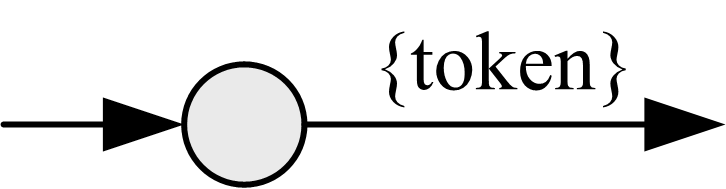
\includegraphics[scale=1.5]{pictures/auto_token}
  \caption{\label{fig:auto_token}Automāts vienai daļiņai}
\end{figure}

Attēlā~\ref{fig:auto_sequence} ir parādīts NGA divu automātu konkatenācijai $e_1 e_2$.
\begin{figure}[H]
  \centering
    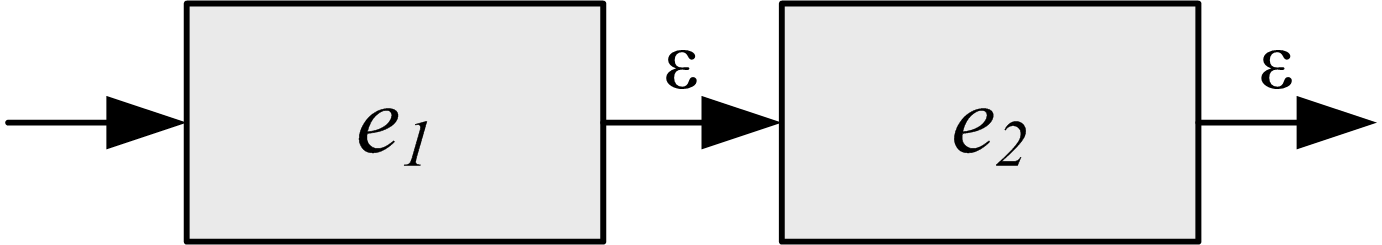
\includegraphics[scale=1.5]{pictures/auto_sequence}
  \caption{\label{fig:auto_sequence}Automāts divu automātu konkatenācijai}
\end{figure}

Attēlā~\ref{fig:auto_or} ir parādīts NGA izvēlei starp diviem automātiem $e_1 | e_2$.
\begin{figure}[H]
  \centering
    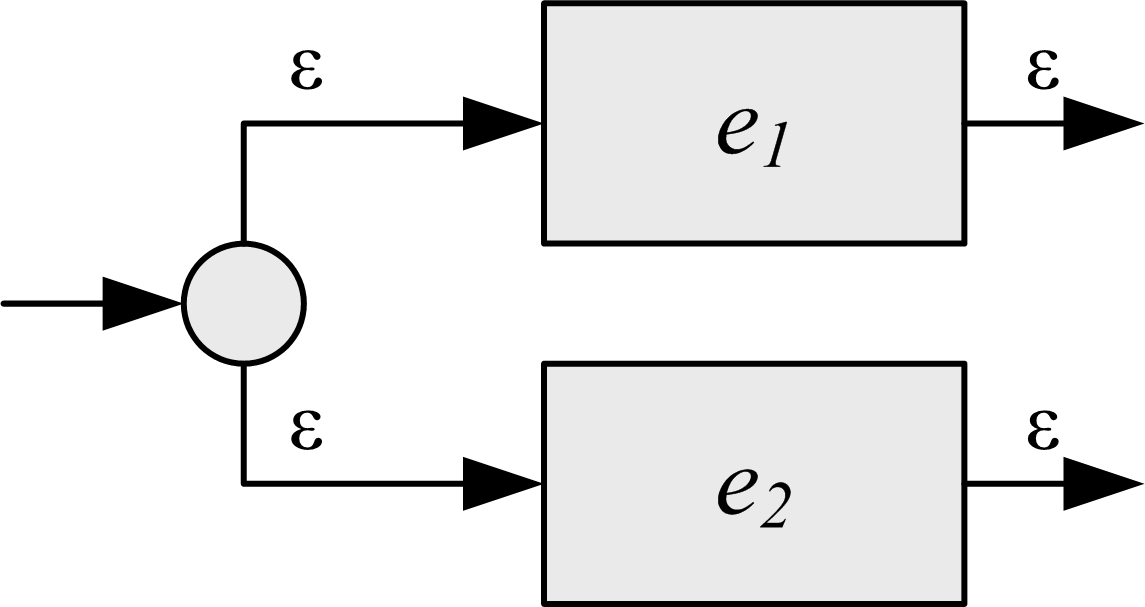
\includegraphics[scale=1.5]{pictures/auto_or}
  \caption{\label{fig:auto_or}Automāts izvēlei starp diviem automātiem}
\end{figure}

Attēlā~\ref{fig:auto_asterisk} ir parādīts NGA priekš konstrukcijas $e_1 *$.
\begin{figure}[H]
  \centering
    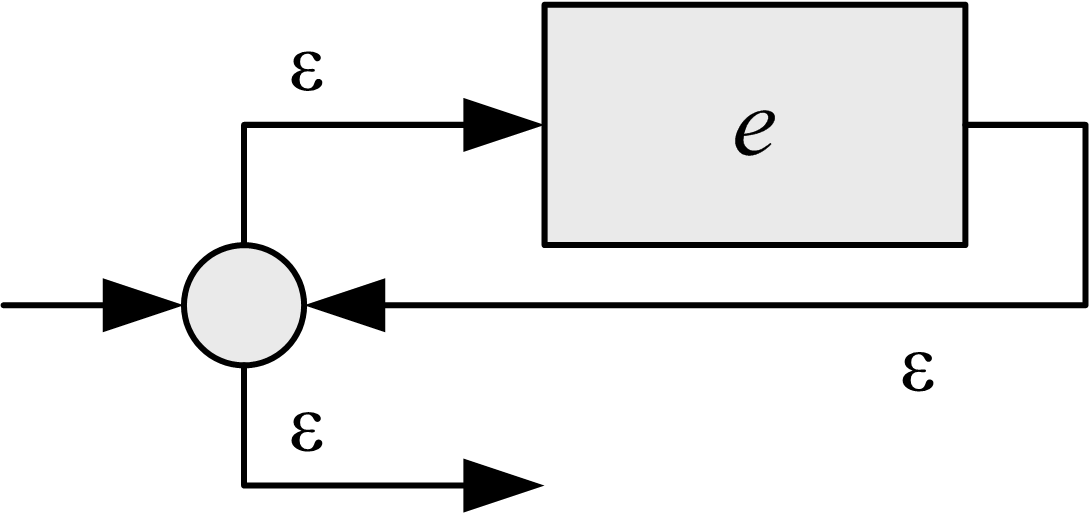
\includegraphics[scale=1.5]{pictures/auto_asterisk}
  \caption{\label{fig:auto_asterisk}Automāts automātu virknei}
\end{figure}

Tālāk šie automāti tiek apvienoti vienā, un beigās tiek pievienots akceptējošais stāvoklis.

Apskatīsim piemēru - izteiksmi \verb/{id} ({real} | {int}) */. Sākumā tiek izveidoti NGA izteiksmes daļām. Attēls~\ref{fig:auto_token_id} parāda NGA priekš \verb|{id}|. Attēls~\ref{fig:auto_or_ex} parāda NGA priekš daļas \verb/{real} | {int}/. Attēls~\ref{fig:auto_asterisk_ex} parāda NGA priekš \verb/({real} | {int}) */.

\begin{figure}[H]
  \centering
    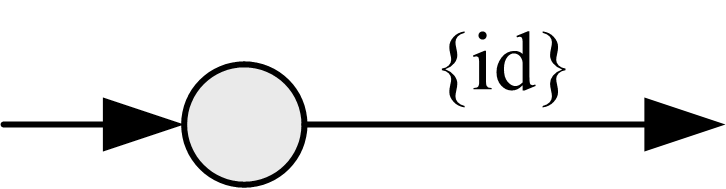
\includegraphics[scale=1.5]{pictures/auto_token_id}
  \caption{\label{fig:auto_token_id}Automāts daļiņai \texttt{\{id\}}}
\end{figure}

\begin{figure}[H]
  \centering
    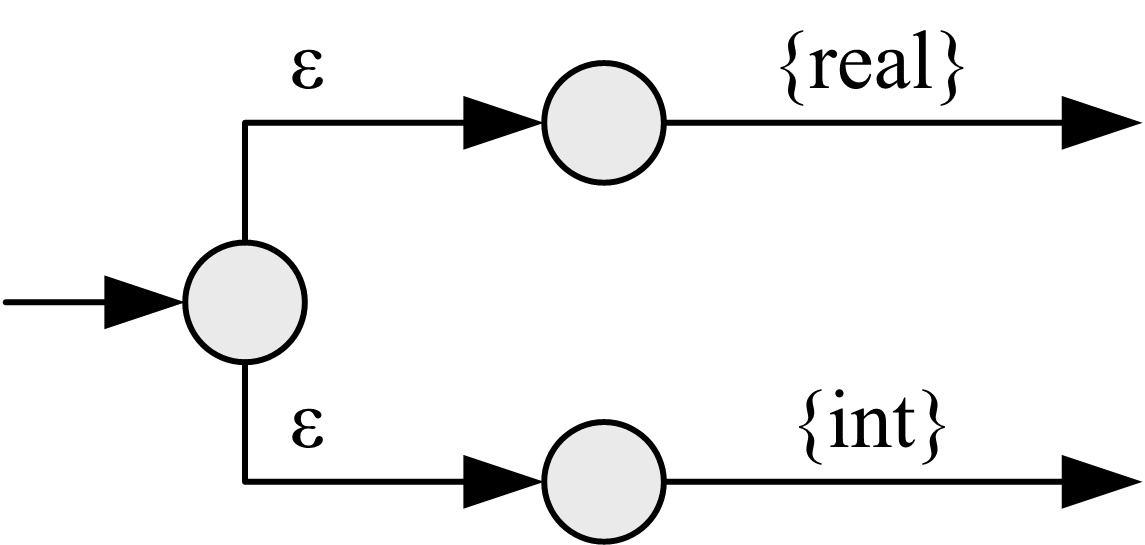
\includegraphics[scale=1.5]{pictures/auto_or_ex}
  \caption{\label{fig:auto_or_ex}Automāts izteiksmei \texttt{\{real\} | \{int\}}}
\end{figure}

\begin{figure}[H]
  \centering
    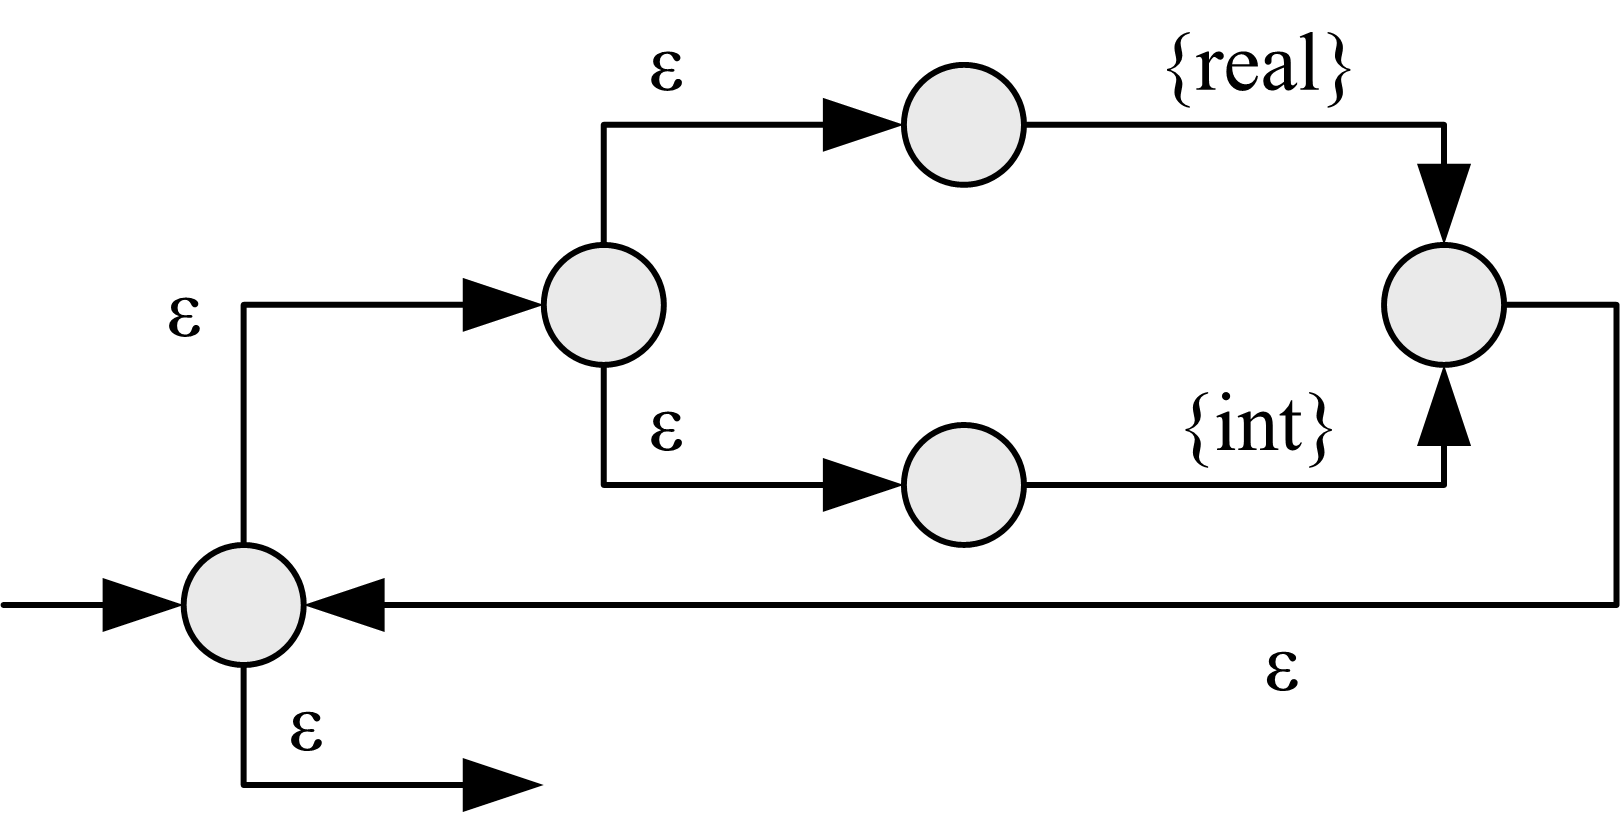
\includegraphics[scale=1.5]{pictures/auto_asterisk_ex}
  \caption{\label{fig:auto_asterisk_ex}Automāts izteiksmei \texttt{(\{real\} | \{int\}) *}}
\end{figure}

Tad izveidotie automāti var tikt savienoti un beigās tiem tiek pievienots akceptējošais stāvoklis (attēls~\ref{fig:auto_full_ex}).

\begin{figure}[H]
  \centering
    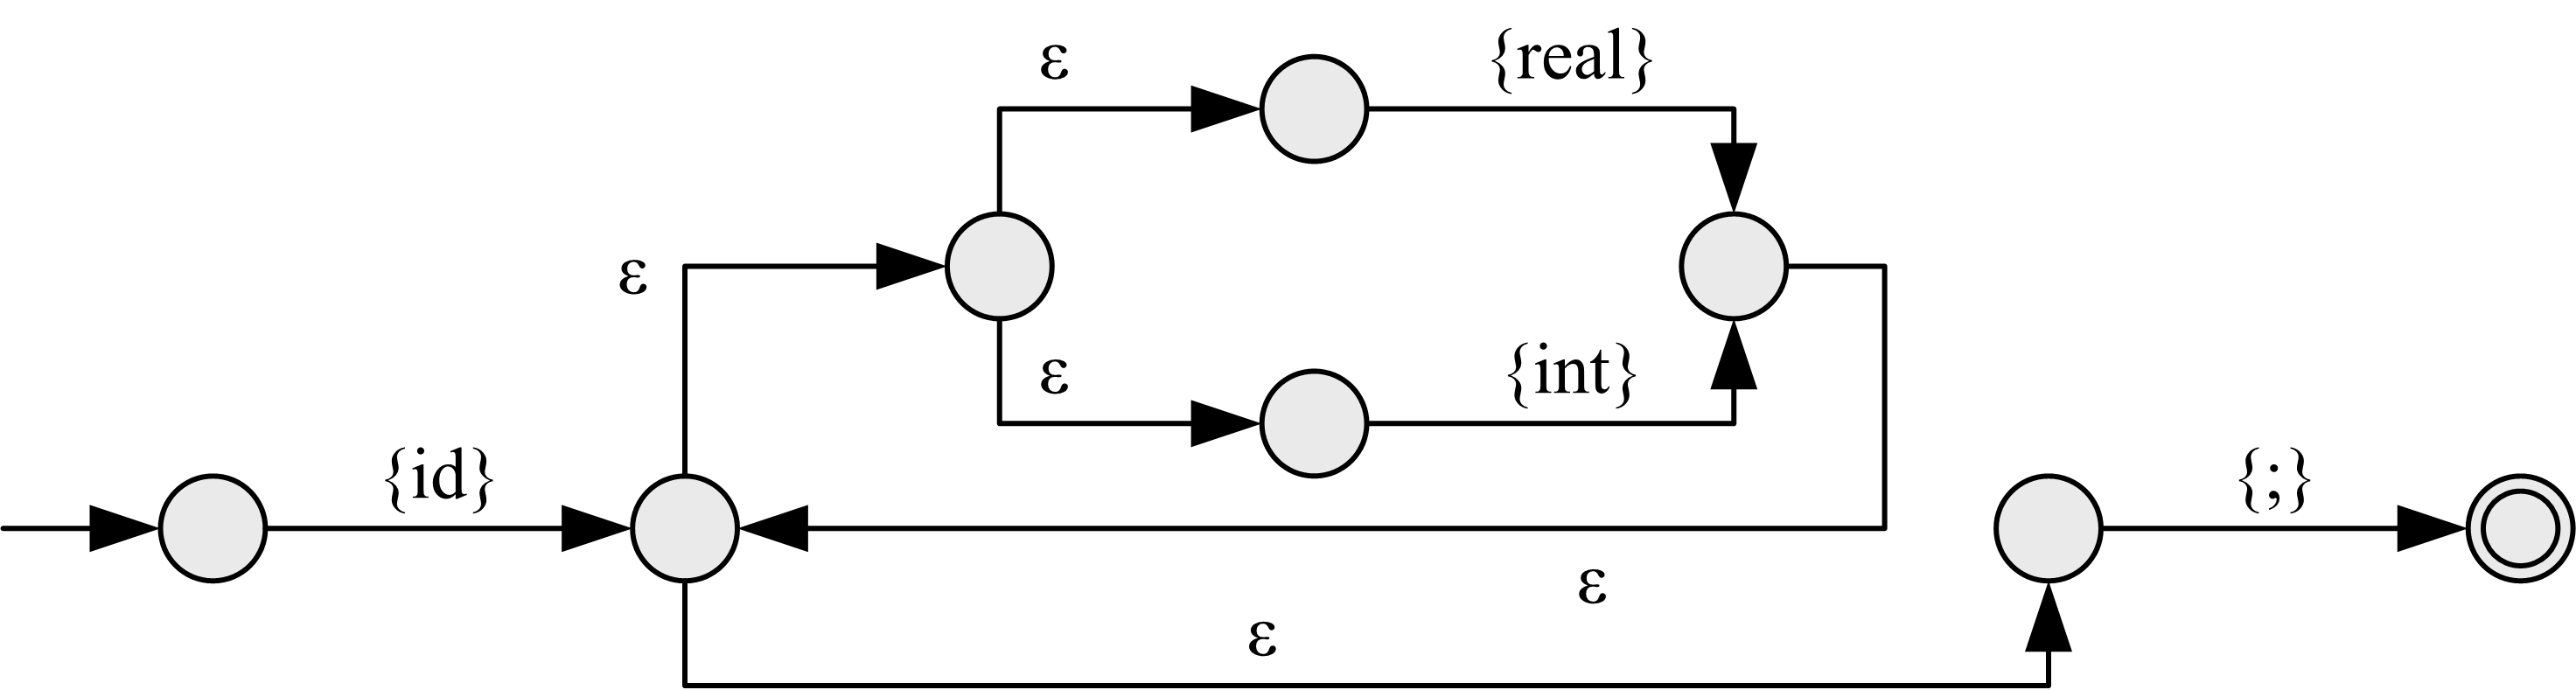
\includegraphics[scale=1.25]{pictures/auto_full_ex}
  \caption{\label{fig:auto_full_ex}Automāts izteiksmei \texttt{\{id\} (\{real\} | \{int\}) * \{;\}}}
\end{figure}

Tā tiek izveidots nedeterminēts automāts katrai regulārai izteiksmei. \cite{Cox:RegexpMatchingFast}, \cite{DragonBook}

\subsubsection{NGA determinizēšana}

Kaut arī daudzām valodām ir vienkāršāk uzbūvēt nedeterminētu galīgu automātu (piemēram, pašām regulārām izteiksmēm tas ir loģiskāk), ir patiess tas, ka katra valoda var tikt aprakstīta gan ar nedeterminētu, gan ar determinētu galīgu automātu. Turklāt, dzīvē sastopamās situācijās DGA parasti satur tik pat daudz stāvokļu, cik ir NGA. Sliktākajā gadījumā, tomēr var gadīties, ka mazākais iespējamais DGA saturēs $m^n$ stāvokļu ($m$ - ieejas alfabēta elementu skaits), kamēr mazākais NGA saturēs $n$ stāvokļus\footnote{Pieņemsim, ka automāta valoda sastāv no diviem simboliem - {0, 1}. Sliktākais gadījums, kad DGA tiešām saturēs $2^n$ stāvokļus attiecībā pret $n$ NGA stāvokļiem, var rasties tad, kad, piemēram, automāta valodā $n$-tais simbols no virknes beigām ir 1. Tad DGA būs jāprot atcerēties pēdējos $n$ simbolus. Tā kā ir divi ieejas alfabēta simboli, automātam ir jāatceras visas to dažādas $2^n$ kombinācijas.}.

Izrādās, ka patiesībā katram NGA eksistē ekvivalents DGA, ko var uzbūvēt ar apakškopu sastādīšanas algoritmu\footnote{Pierādījumu tam, ka uzbūvētais DGA tik tiešām akceptē to pašu valodu, ko NGA, sk.  \cite{Hopcroft:IntroAutomataTheory}, teorēma 2.11.}. Vadošā doma šī algoritmā ir tas, ka katrs determinētā galīgā automāta (DGA) stāvoklis ir kādu NGA stāvokļu kopa. Pēc ieejas virknes $a_1, a_2, ..., a_n$ ielasīšanas DGA atrodas stāvoklī, kas atbilst NGA stāvokļu kopai, kuru var sasniegt apstaigājot virkni $a_1, a_2, ..., a_n$.

Algoritms ir paņemts no~\cite{DragonBook}.

\paragraph*{Algoritms 1: NGA transformēšana uz DGA}
\subparagraph{Ieeja:}NGA $N$.
\subparagraph{Izeja:}DGA $D$, kas ir ekvivalents $N$.
\subparagraph{Algoritms:} Sākumā algoritms konstruē pāreju tabulu priekš $D$. Katrs $D$ stāvoklis ir $N$ stāvokļu kopa, tātad tabula tiek konstruēta tā, lai $D$ simulētu vienlaikus visas pārejas, ko var izpildīt $N$, saņemot kādu ieejas virkni. Lai automāts kļūtu determinēts, ir nepieciešams atbrīvoties no iespējas atrasties dažos stāvokļos vienlaikus. Tātad vajag atbrīvoties no $\varepsilon$-pārejām, un no daudzkārtīgām pārejām no viena stāvokļa pa vienu ieejas simbolu.

Tabulā~\ref{fig:NGAoperations} var redzēt divas funkcijas, kas ir nepieciešamas NGA apstrādes izpildei. Šīs funkcijas no NGA stāvokļiem un pārejām veido jaunas stāvokļu kopas, kuras veidos DGA stāvokļus.

\begin{table}[H]
  \caption{NGA apstaigāšanas funkcijas}
  \centering
  \begin{tabular}{|c|p{350pt}|}
    \hline
    Funkcija & Apraksts \\ \hline
    $\varepsilon-closure (T)$ & 
    NGA stāvokļu kopa, kas ir sasniedzama lietojot tikai $\varepsilon$-pārejas no visiem stāvokļiem no kopas $T$. \\ \hline
    $move (T, a)$ & 
    NGA stāvokļu kopa, kas ir sasniedzama lietojot pārejas pa simbolu $a$ no visiem stāvokļiem no kopas $T$. \\
    \hline
  \end{tabular}
\label{fig:NGAoperations}
\end{table}

Ir nepieciešams apstrādāt visas tādas $N$ stāvokļu kopas, kuras ir sasniedzamas, $N$ saņemot kaut kādu ieejas virkni. Indukcijas bāzes pieņēmums ir tas, ka pirms darbības uzsākšanas $N$ var atrasties jebkurā no stāvokļiem, kurus var sasniegt pārejot pa $\varepsilon$ bultiņām no $N$ sākuma stāvokļa. Ja $s_0$ ir $N$ sākuma stāvoklis, $D$ sākuma stāvoklis būs $\varepsilon-closure (set (s_0))$. Indukcijai pieņemam, ka $N$ var atrasties $T$ stāvokļu kopā pēc virknes $x$ ielasīšanas. Tad, ja $N$ ielasīs nākamo simbolu $a$, tad $N$ var pārvietoties jebkura no stāvokļiem $move (T, a)$. Taču pēc $a$ ielasīšanas var notikt vēl dažas $\varepsilon$-pārejas, tāpēc pēc virknes $xa$ ielasīšanas $N$ var atrasties jebkurā no stāvokļiem $\varepsilon-closure (move (T, a))$. Attēls~\ref{fig:det_algorithm} parāda pseido-kodu algoritmam, kā šādā veidā var tikt uzkonstruēti visi DGA stāvokļi un tā pāreju tabula.

Automāta $D$ sākuma stāvoklis ir $\varepsilon-closure(set(s_0))$, bet $D$ akceptējošie stāvokļi ir visas tās NGA stāvokļu kopas, kas satur vismaz vienu akceptējošu stāvokli. $Dstates$ ir jauna automāta $D$ stāvokļu saraksts un $Dtran$ ir stāvokļu pāreju tabula.

\begin{figure}[H]
  \begin{algorithmic}
  \State initially, $\varepsilon-closure (set (s_0))$  is the only state in $Dstates$, and is unmarked
  \While{there is an unmarked state $S$ in $Dstates$}
      \State mark $S$
      \For{each available path $t$ from $S$} 
          \State $U = \varepsilon-closure (move (S, a))$
          \If {$U$ is not in $Dstates$}
              \State add $U$ as an unmarked state to $Dstates$
          \EndIf
          \State $Dtran [S, a] = U$;
      \EndFor
  \EndWhile
  \end{algorithmic}
  \caption{\label{fig:det_algorithm}Automāta determinēšanas algoritms}
\end{figure}

\subparagraph{Sarežģītība:} Sarežģītības novērtējums šīm algoritmam ir diezgan nepatīkams. Sliktākajā gadījumā tas būs $O(m^{n+1})$, kur $n$ ir NGA stāvokļu daudzums un $m$ ir ieejas alfabēta simbolu skaits. Algoritms var uzģenerēt līdz $m^n$ DGA stāvokļiem, katram no kuram ir $m$ pārejas. Taču parasti tas tā nenotiek un DGA stāvokļu skaits ir līdzīgs NGA stāvokļu skaitam, un algoritma sarežģītība ir $O(n*m)$. \cite{DragonBook, Hopcroft:IntroAutomataTheory}

\subsubsection{\label{sbsbs:prot_minimization}DGA minimizēšana}

Izveidotais determinēts galīgs automāts var būt neoptimāls pēc stāvokļu skaita. Bet no šī skaitļa ir atkarīgs tālāko soļu izpildes ātrums. Tātad ir nepieciešams izveidot automātu, kas atpazīs to pašu valodu un saturēs minimālu iespējamu stāvokļi skaitu.

Var pierādīt, ka katram automātam eksistē ekvivalents minimāls automāts\footnote{Šī fakta pierādījumu sk.~\cite{Bassino:ComplexityMinimization}}. Vēl vairāk, ja eksistē 2 dažādi automāti ar vienādu stāvokļu daudzumu, kas atpazīst vienu un to pašu valodu, tad tie ir vienādi līdz stāvokļu nosaukumiem\footnote{Tā kā stāvokļu nosaukumi neietekmē automāta darbību, divi automāti tiek saukti par vienādiem līdz pat stāvokļu nosaukumiem, ja viens no tiem var tikt pārveidots otrajā vienkārši pārsaucot to stāvokļus.}.

Tālāk teiksim, ka virkne $x$ atšķir stāvokļu $s$ no stāvokļa $t$ tad, kad tikai viens stāvoklis, ko var sasniegt no $t$ un $s$ pa $x$ ir akceptējošs. Tātad divi stāvokļi ir atšķirami tad, kad eksistē tāda virkne, kas viņus atšķir. Jebkurš akceptējošs stāvoklis ir atšķirams no jebkura neakceptējoša stāvokļa ar tukšu virkni (stāvoklis nevar būt akceptējošs un neakceptējošs vienlaikus). Divi neatšķirami stāvokļi ir ekvivalenti\footnote{\cite{Hopcroft:IntroAutomataTheory} nodaļa 4.4}.

Algoritms ir paņemts no~\cite{DragonBook}.

\paragraph*{Algoritms 2: DGA minimizēšana}
\subparagraph{Ieeja:}DGA $D$.
\subparagraph{Izeja:}Jauns DGA $D'$, kas ir minimāls un ekvivalents $D$.
\subparagraph{Algoritms:} 

Minimizēšanas algoritma vadošā doma ir sadalīt automātu neatšķiramos stāvokļu grupās. Tas izveido ekvivalentu stāvokļu grupas, kas tālāk var tikt apvienotas vienā, izveidojot minimāla automāta stāvokļus.

Minimizēšanas gaitā automāta stāvokļi tiek sadalīti grupās, ko uz doto brīdi algoritms nevar atšķirt. Jebkuri divi stāvokļi no dažādām grupām ir atšķirami. Katrā nākamajā algoritma iterācijā eksistējošās grupas tiek sadalītas mazākajās grupās, gadījumā, ja kādā grupā parādās atšķirami stāvokļi. Algoritms apstājas līdz ko neviena grupa nevar tikt sadalīta sīkāk.

Pirms algoritms uzsāk darbu, stāvokļi tiek sadalīti divās grupās - akceptējošie stāvokļi un neakceptējošie stāvokļi. Šo grupu stāvokļi ir atšķirami ar tukšu virkni. Tālāk tiek pa vienai apstrādātas grupas no pašreizējā sadalījums. Katrai grupai tiek pārbaudīts, vai tās stāvokļi var tikt atšķirti ar kādu ieejas simbolu - vai kāds no ieejas simboliem noved uz divām vai vairākām dažādam stāvokļu grupām. Ja tādi simboli eksistē, tiek izveidotas jaunas grupas, tādas, ka divi stāvokļi atrodas vienā grupā tad un tikai tad, ja tie aiziet uz vienādām grupām pa vienādiem simboliem. Process ir atkārtots visām pašreizējā sadalījuma grupām, tad atkal jaunam sadalījumam, kamēr neviena no grupām vairs nevar tikt sadalīta.

Attēls~\ref{fig:min_algorithm} parāda minimizēšanas algoritmu pseido-kodā.

\begin{figure}[H]
  \begin{algorithmic}
  \State initially, partitioning $\Pi$ contains two groups, $F$ and $S-F$, the accepting and nonaccepting states of $D$, $\Pi_{new}$ is empty
  \While{$\Pi_{new}$ is not equal to $\Pi$}
      \State $\Pi_{new} = \Pi$
      \For{each group $G$ of $\Pi$}
          \State partition $G$ into subgroups such that two states $s$ and $t$ are in the same subgroup if and only if for all input symbols $a$, states $s$ and $t$ have transitions on $a$ to states in the same group of $\Pi$
          \State replace $G$ in $\Pi_{new}$ by the set of all subgroups formed
      \EndFor
  \EndWhile
  \State $\Pi_{final} = \Pi$
  \end{algorithmic}
  \caption{\label{fig:min_algorithm}Automāta minimizēšanas algoritms}
\end{figure}

Tālāk paliek apstrādāt jaunizveidotās stāvokļu grupas izveidojot jaunu determinētu automātu. Lai to izdarītu, no katras sadalījuma $\Pi_{final}$ grupas tiek izvēlēts grupas pārstāvis. Grupu pārstāvji izveidos jaunus stāvokļus automātam $D'$. Pārējās komponentes minimālam automātam $D'$ tiks izveidotas sekojoši:
\begin{enumerate}
\item Automāta $D'$ sākuma stāvoklis ir pārstāvis tai grupai, kura satur automāta $D$ sākuma stāvokli.
\item Automāta $D'$ akceptējošie stāvokļi ir pārstāvji tām grupām, kuras satur automāta $D$ akceptējošos stāvokļus. Katra no grupām satur vai nu tikai akceptējošus, vai nu tikai neakceptējošus stāvokļus, jo algoritma darba gaitā jaunās grupas tika izveidotas tikai sadalot jau eksistējošas grupas, bet sākuma sadalījums atdalīja šīs stāvokļu klases.
\item Pieņemsim, ka $s$ ir kādas $\Pi_{final}$ grupas $G$ pārstāvis, un automāts $D$ no stāvokļa $s$ pa ieejas simbolu $a$ pāriet uz stāvokli $t$. Pieņemsim, ka $r$ ir grupas $H$ pārstāvis, $H$ satur $t$. Tad automātā $D'$ ir pāreja no stāvokļa $s$ uz stāvokli $r$ pa ieejas simbolu $a$.
\end{enumerate}

\subparagraph{Sarežģītība:}
Šī algoritma sarežģītība sliktākajā gadījumā ir $O(n^2)$, kur $n$ ir sākotnējā automāta stāvokļu daudzums. Tomēr vidēji algoritma darbības sarežģītība ir $O(n$ log $n)$. \cite{Bassino:ComplexityMinimization}

\subsubsection{DGA apvienošana}

Kā jau bija teikts agrāk, lai samazinātu sakrišanu meklēšanas laiku, tika izvēlēts apvienot visus meklēšanas automātus vienā. Tā kā makro atnāk pa vienam dažādās vietās programmas kodā un var sākt uzreiz tikt lietotas, nav iespējams gaidīt kamēr sakrāsies vairāki automāti apvienošanai. Tikko parādās divi automāti tie tūlīt pat tiek apvienoti vienā sistēmā. Tālāk, kad parādās citi makro, to automāti tiek pievienoti jau eksistējošam.

Algoritms pēc savas būtības ir determinēšanas algoritma adaptācija. Vienīgais uzņēmums ir tas, ka nevienā no automātiem neeksistē $\varepsilon$-pārejas. Tātad tas, no kā vajag atbrīvoties, ir pārejas pa vienu un to pašu simbolu uz diviem dažādiem stāvokļiem. Tas tiek darīts apvienojot divus stāvokļus no dažādiem automātiem. 

\paragraph*{Algoritms 3: Divu DGA apvienošana}
\subparagraph{Ieeja:}DGA $D_1$ un $D_2$.
\subparagraph{Izeja:}Jauns DGA $D'$, kas apvieno $D_1$ un $D_2$.
\subparagraph{Algoritms:} 

Algoritms sāk darbu apvienojot $D_1$ un $D_2$ sākuma stāvokļus. Šo stāvokļu kombinācija veido automāta $D'$ sākuma stāvokli. Tālāk algoritms apskata visas iespējamas pārejas no katra no kombinētiem stāvokļiem un apvieno to rezultātus jaunajos stāvokļos. 

Apskatīsim piemēru automātu apvienošanai. Attēls~\ref{fig:auto_m_1} parāda determinētu minimālu automātu priekš regulārās izteiksmes \verb|{id}* {int}*|. Tas satur divus stāvokļus, \verb|a| un \verb|b|, kuri abi ir akceptējoši. Attēls~\ref{fig:auto_m_2}, savukārt, parāda DGA priekš izteiksmes \verb|{id} {real}* {int}|.

\begin{figure}[H]
  \centering
    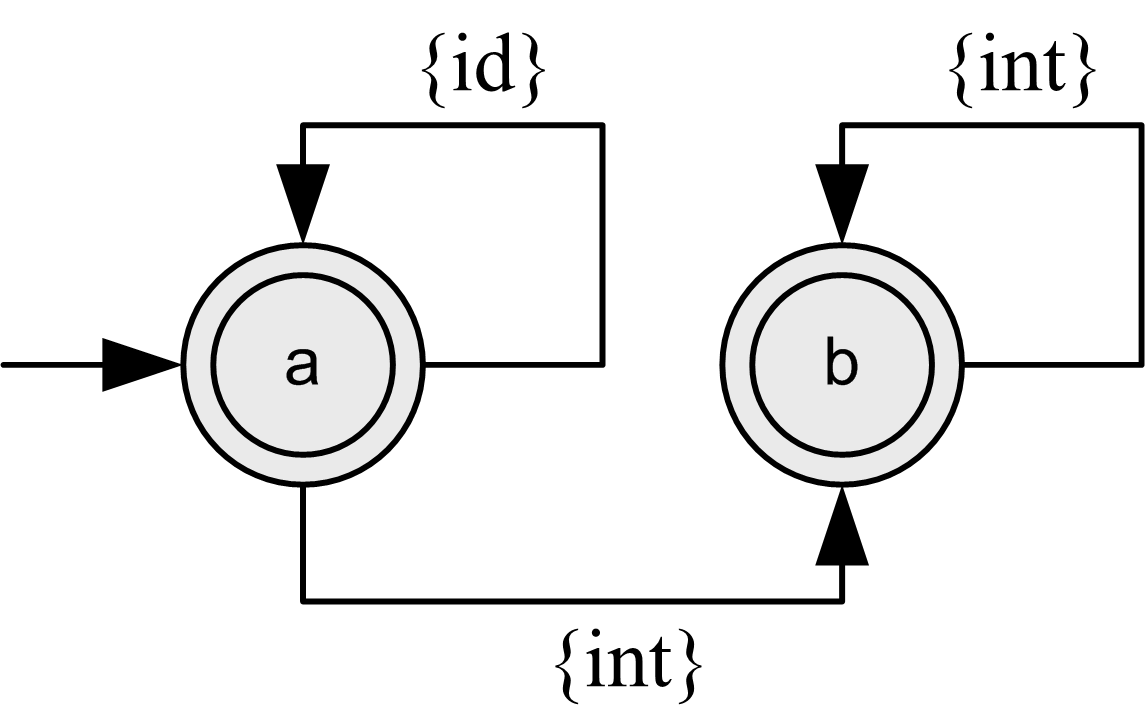
\includegraphics[scale=1.5]{pictures/auto_m_1}
  \caption{\label{fig:auto_m_1}Automāts izteiksmei \texttt{\{id\}* \{int\}*}}
\end{figure}

\begin{figure}[H]
  \centering
    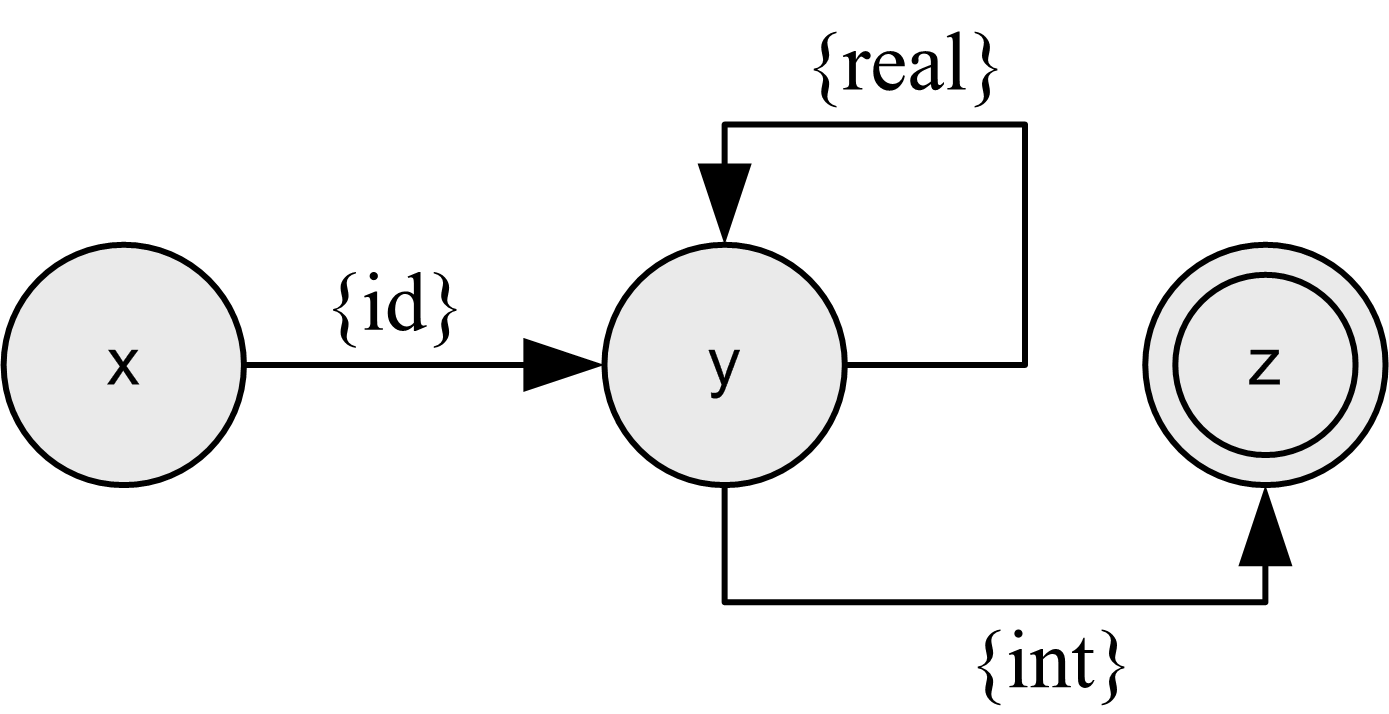
\includegraphics[scale=1.5]{pictures/auto_m_2}
  \caption{\label{fig:auto_m_2}Automāts izteiksmei \texttt{\{id\} \{real\}* \{int\}}}
\end{figure}

To apvienotais automāts ir parādīts attēlā~\ref{fig:auto_merge}.

\begin{figure}[H]
  \centering
    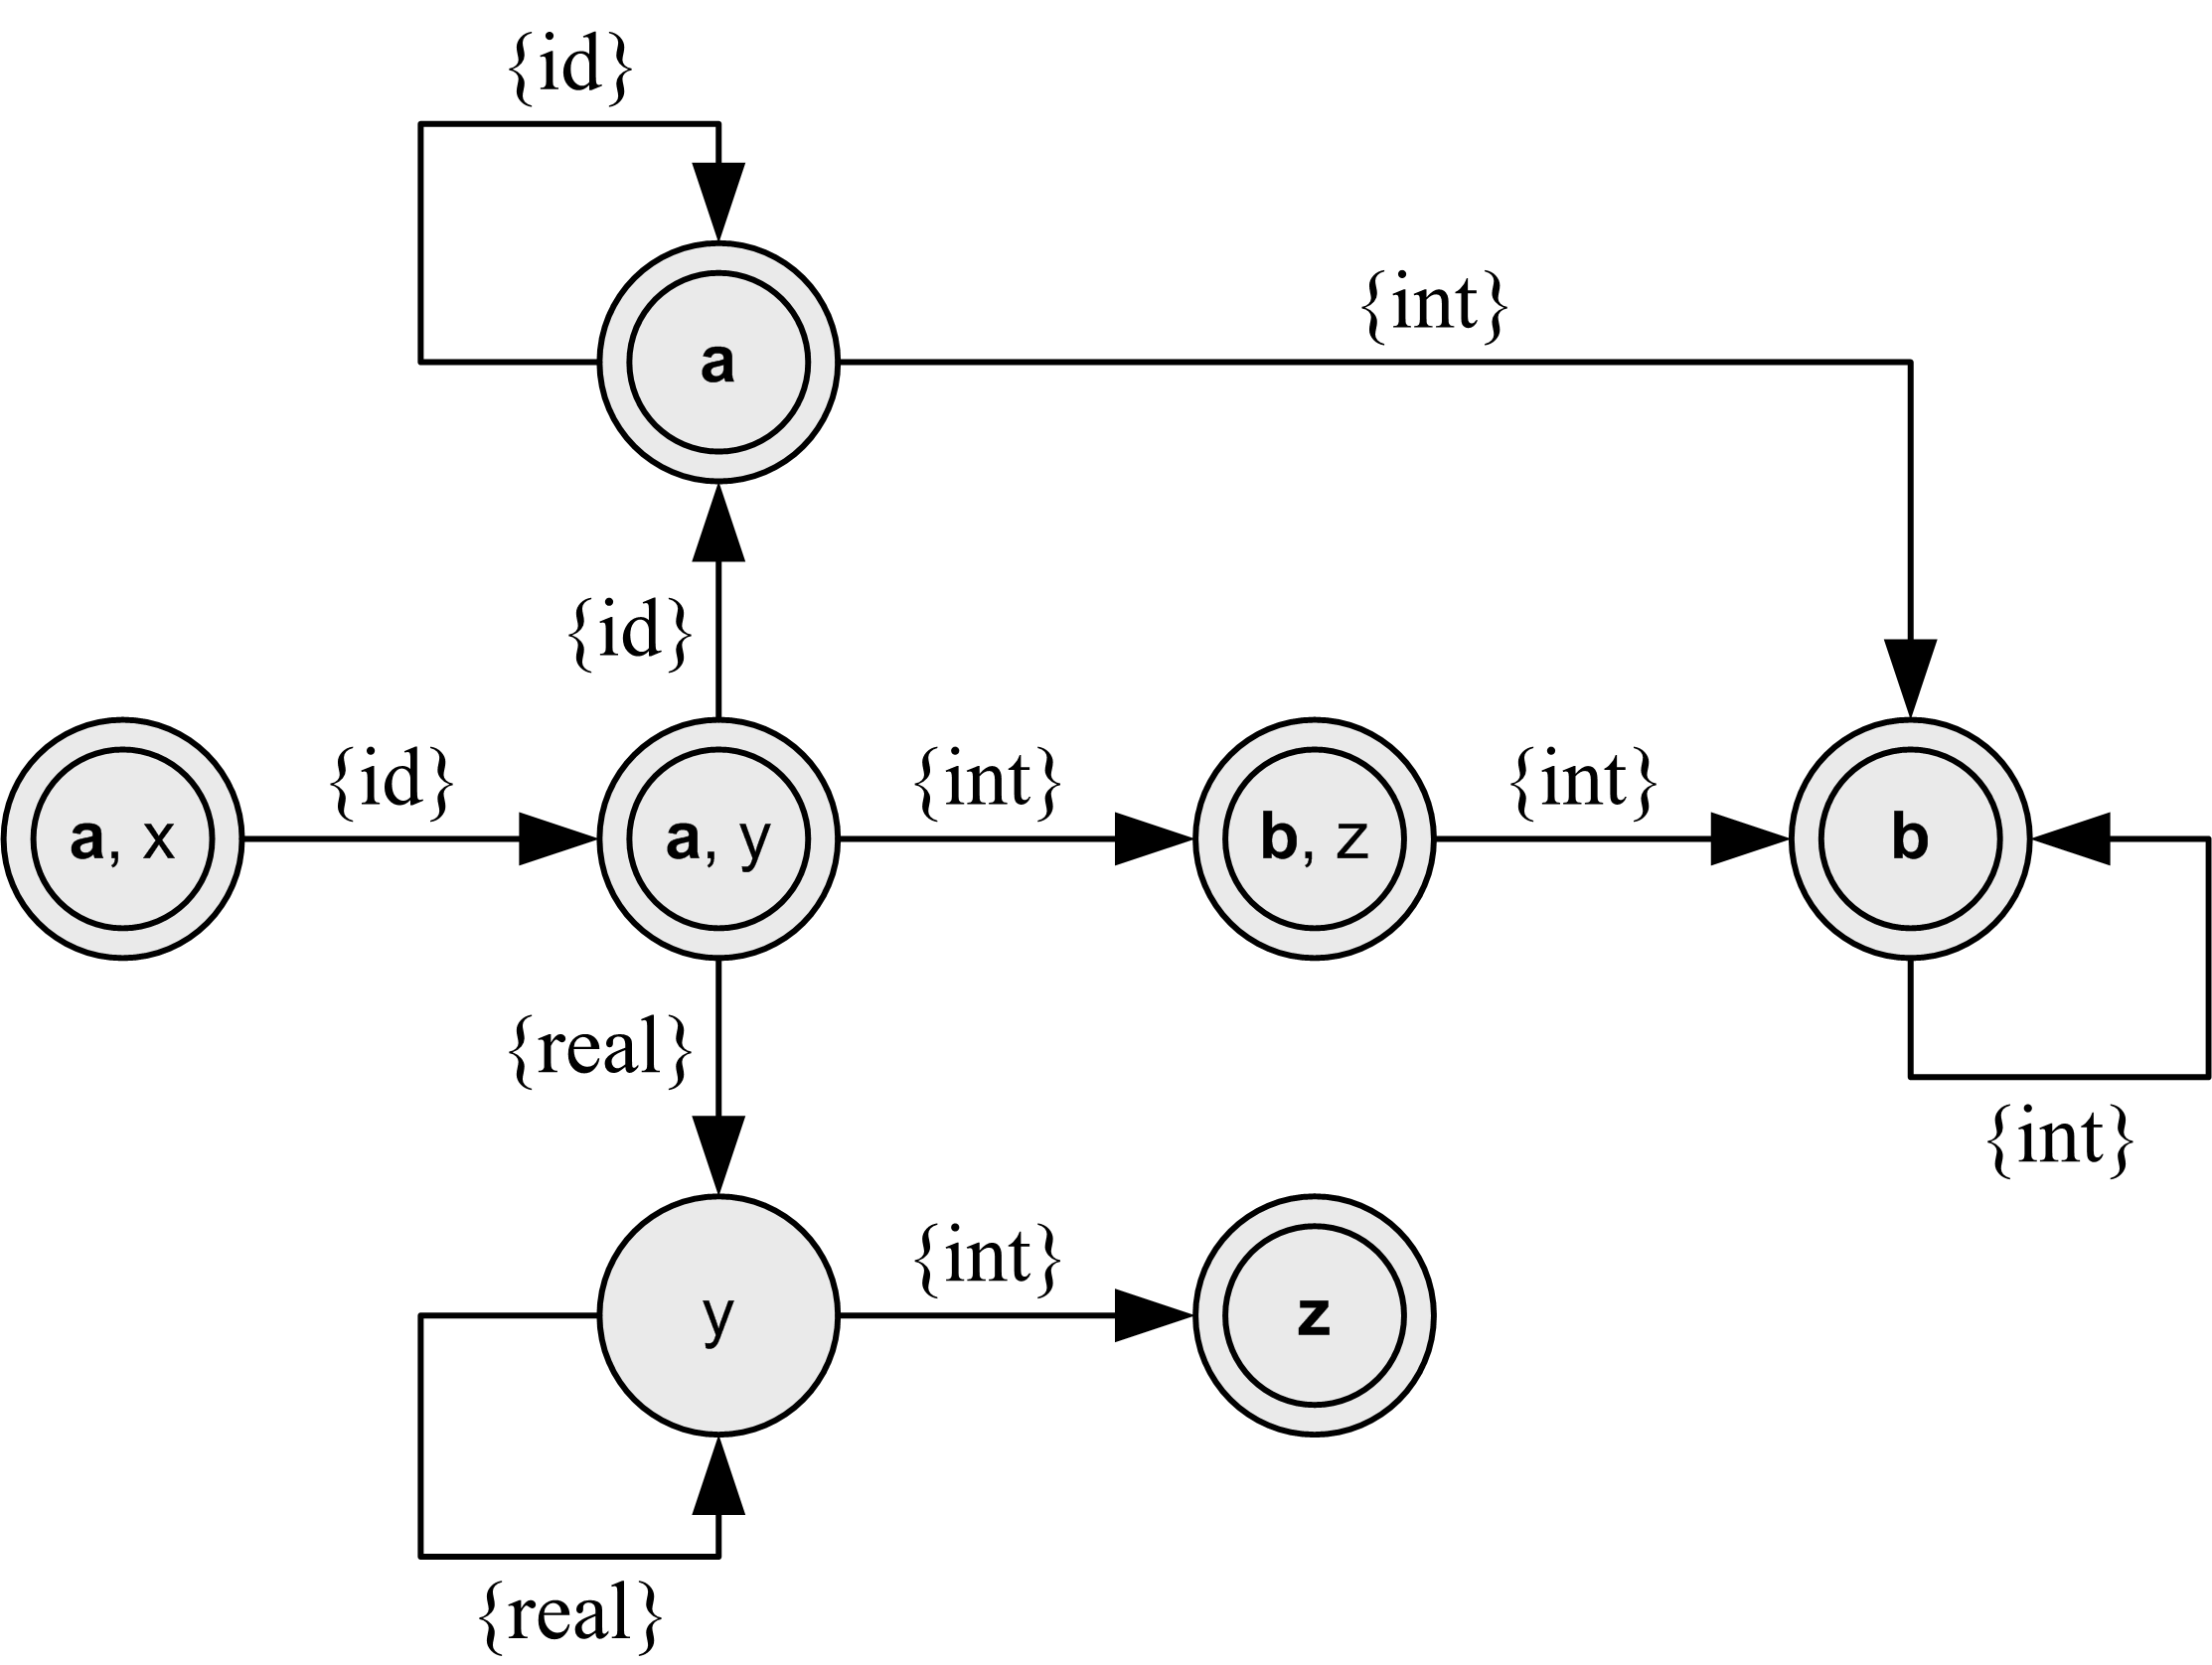
\includegraphics[scale=1.5]{pictures/auto_merge}
  \caption{\label{fig:auto_merge}Automāts izteiksmju \texttt{\{id\}* \{int\}*} un \texttt{\{id\} \{real\}* \{int\}} apvienojumam}
\end{figure}

Attēls~\ref{fig:uni_algorithm} parāda apvienošanas algoritmu pseido-kodā. $s_0$ ir jaunā automāta $D'$ sākuma stāvoklis, $r_0$ ir $D_1$ sākuma stāvoklis un $t_0$ ir $D_2$ sākuma stāvoklis. $Dstates$ ir automāta $D'$ stāvokļu saraksts, $Dtran$ ir $D'$ pāreju tabula. Funkcija $move (S, t)$ atgriež tos stāvokļus, uz kuriem var nokļūt no $S$ pa daļiņu $t$. Tā kā parasti $S$ sastāv no diviem stāvokļiem $r_i$ un $t_i$, tā atgriež pārejas rezultātu no katra no tiem. Rezultāts arī var būt tikai viens stāvoklis, gadījumā, ja no kāda $r_i$ un $t_i$ neeksistē pāreja pa doto daļiņu.

\begin{figure}[H]
  \begin{algorithmic}
  \State initially, $s_0 = (r_0, t_0)$ is the only state in $Dstates$, and is unmarked
  \While{there is an unmarked state $S$ in $Dstates$}
      \State mark $S$
      \For{each available move $t$ from $S$} \Comment{$S$ is a combination of some states $r_i$ and $t_i$ of $D_1$ and $D_2$, although it might be just a single state from one of the automata.}
          \State $U = move (S, t)$
          \If {$U$ is not in $Dstates$}
              \State add $U$ as an unmarked state to $Dstates$
          \EndIf
          \State $Dtran [S, t] = U$;
      \EndFor
  \EndWhile
  \end{algorithmic}
  \caption{\label{fig:uni_algorithm}Divu automātu apvienošanas algoritms}
\end{figure}

\subparagraph{Sarežģītība:}
Šī algoritma sarežģītība ir $O(n*m*l)$, kur  $n$ ir pirmā automāta stāvokļu daudzums, $m$ ir otrā automāta stāvokļu daudzums, un $l$ maksimāls pāreju daudzums no katra no stāvokļiem.

\subsubsection{Tvērumu apstrāde}

Viena no galvenām šīs sistēmas īpašībām ir iespēja atšķirt programmatūras tvērumus. Ir dažādi veidi, kā var izveidot automātus, kas atšķirtu atsevišķu tvērumu makro. Viens no veidiem varētu būt tāds - katram tvērumam izveidot automātu rindu, kur tvērumam specifiskākie automāti tiks pārbaudīti pirmie. Bet gadījumā, ja ir $n$ iekļautie tvērumi un nepieciešamais makro ir atrodams pirmajā automātā, būs jāizpilda vismaz $n$ meklēšanas, līdz ko pareizais šablons tiks atrasts. Atstājot tikai vienu aktīvu automātu vienā laika brīdī, arī ir dažas iespējas. Varētu visus šablonus likt vienā automātā kopā, un tad pēc izejas no tvēruma attiecīgos šablonus dzēst ārā. Tas nozīmētu, ka katram tvērumam jāatceras makro, kas tika pievienoti, un jāprot dzēst daļu no stāvokļiem ārā no automāta. Bet stāvokļu dzēšana ir laikietilpīga operācija, jo tās izpildīšanai būs nepieciešams apstaigāt visu lielo automātu, dzēšot no tā nevajadzīgos stāvokļus.

Tāpēc tika izvēlēta sekojoša pieeja. Ja prototips darba gaitā sastapās ar tvēruma sākuma simbolu, tas izveido eksistējošā automāta kopiju un ieliek to kaudzē. Tad automātam tiek pievienotas tvēruma makro. Izejot no tvēruma tā specifiskais automāts tiek izmests ārā un darbs tiek turpināts ar pēdējo automātu no kaudzes, kas atbilst iepriekšējam tvērumam. Šādā veidā jebkurā laika brīdī aktīvs ir tikai viens sakrišanu meklēšanas automāts.

\subsubsection{Sakrišanu meklēšana}
Sakrišanu meklēšana NGA sliktākajā gadījumā būs ar sarežģītību $O(n^2*l)$, kur $n$ ir NGA stāvokļu skaits un $l$ - pārbaudāmās virknes elementu skaits. Tas var notikt, kad visi NGA stāvokļi ir aktīvi vienā laika brīdī, un no katra no tiem eksistē $n$ pārejas pa ieejas simbolu uz visiem automāta stāvokļiem.

Tīrā DGA gadījumā sakrišanu pārbaude katram ieejas elementam ir $O(l)$, kur $l$ ir pārbaudāmās virknes garums. 

Diemžēl pilnībā lineāra laika sakrišanu meklēšana nav iespējama tādēļ, ka prototips dod iespēju lietot makro ar daļiņu vērtībām. Piemēram, eksistē 2 makro, viens no kuriem gaida daļiņu \verb|{id}|, un otrs \verb|{id:foo}|. Gadījumā, kad sakrišanu meklēšanas procesā parādās daļiņa \verb|{id:foo}|, automātam nav iespējas izsecināt, kurš no ceļiem novedīs pie garākas sakritības. Tādēļ tas iet pa abiem ceļiem vienlaikus, saglabājot abus stāvokļus.

Kaut arī tas ievieš nenoteiktību, tā var parādīties tikai augstāk minētā gadījumā un izveidot ne vairāk ka 2 ceļus vienlaikus. Tātad kaut arī nenoteiktība pastāv, tai ir ļoti maza iespējamība un maza ietekme uz sakrišanu meklēšanas laiku.

\subsection{\label{sbs:prot_problems}Izņēmumi}

\subsubsection{Produkcijas}

Prototipā pagaidām nav implementēta apstrādes dalīšana pa gramatikas produkcijām, visas regulārās izteiksmes ir sapludinātas vienā automāta. Regulāro izteiksmju dalīšana pa tipiem tiks ieviesta vēlāk, kad tiks uzsākta integrācija un sadarbība ar reālu parsētāju. Tā varētu tikt implementēta līdzīgi tam, kā tiek realizēti konteksti - pa vienam sapludinātam automātam priekš katra produkcijas tipa.

\subsubsection{Daļiņu klašu mantošana}

Sistēmai ir minimāla informācijas par valodas gramatiku, tai ir zināšanas tikai par daļiņu un produkciju nosaukumiem. Tieši tāpēc daļiņa \verb|{real}| netiks uztverta ka \verb|{expr}|, kaut arī racionāls skaitlis ir izteiksme. Tā kā sistēmai jābūt pēc iespējas vairāk neatkarīgai no valodas gramatikas, lai būtu universālākai, šī hierarhija nav iekodējama transformāciju sistēmā. To ir jānodrošina parsētājam, attiecīgi apstrādājot daļiņas apkopojot to nozīmi un veidojot saskarni priekš šablonu sistēmas.% Par to arī būs jārūpējas sistēmas lietotājam rakstot savas makro izteiksmes.

\subsubsection{Regulārās izteiksmes daļu grupēšana}

Tādēļ, ka aprakstītā pieeja mēģina pēc iespējas minimizēt meklēšanas laiku, tā neatļauj veidot atrasto daļiņu grupēšanu, kā tas ir parasti pieņemts regulārās izteiksmēs. Daļiņu grupēšana un atpakaļnorādes (\emph{backreferences}) uz daļiņu grupām nav atļautas.

Tomēr ja parādīsies nepieciešamība, ir apskatīta arī pieeja, kas dos šādu iespēju. Tas varētu tikt izpildīts, determinējot tikai automāta stāvokļus grupu iekšienē, pēc tam ar $\varepsilon$-pārejām secīgi savienojot grupu automātu akceptējošus un sākuma stāvokļus. Automāts būs determinēts tikai grupu ietvaros, bet tad būs pieejamas atrasto daļiņu grupas. Tomēr šāda pieeja neatļaus sapludināt dažus automātus vienā, jo sapludināšanas procedūra sabojās grupēšanu.

\subsubsection{Sapludinātā automāta minimizēšana}

Automātu minimizēšana ir diezgan darbietilpīga operācija, tāpēc tā tiek izpildīta tikai uz atsevišķiem automātiem. Apvienotais visu šablonu automāts var nebūt minimāls, jo dažādu minimālu automātu apvienošana negarantē šo faktu. Bet tā kā apvienota automāta stāvokļu daudzums var būt ļoti liels, minimizēšanas izpilde var būt neefektīva. Tā kā minimizēšana samazina tikai automāta aizņemto vietu, nevis apstaigāšanas laiku, to šajā gadījumā var izlaist. Sapludinātā automāta minimizēšanu apgrūtina arī tas fakts, ka to stāvokļus vajadzēs atšķirt arī pēc tā fakta, kāds no šabloniem ir akceptēts, nevis tikai pēc tā, vai stāvoklis ir akceptējošs.

\subsection{\label{subsec:solution_optimization}Optimizācijas iespējas}

Regulāro izteiksmju optimizēšana uz doto brīdi netiek izpildīta, jo to ir vērts izpildīt uz regulārām izteiksmēm, kas tiks lietoti daudzas reizes. Darba apskatītā situācijā regulārās izteiksmes tiks lietotas tikai vienas programmas ietvaros un to optimizēšanai nav īpašas jēgas. Tomēr bez reāliem piemēriem nevar izšķirt, vai tas izveidos būtisku paātrinājumu šādā konkrētā gadījumā vai nē. Dažas regulāro izteiksmju pārrakstīšanas pieejas, kas varētu būt lietotas tālākā izstrādē ir aprakstītas \cite{Yu:FMR}.

Dažreiz divu automātu sapludināšana var izraisīt pārāk lielu stāvokļu daudzumu rašanos. Ja reālajā situācijā tas ietekmēs apstrādes laiku, vai parādīsies nepieciešamība ierobežot automāta aizņemto laiku, var apskatīt iespēju glabāt dažus automātus ar stāvokļu skaitu robežu, nevis tikai vienu. Šāda pieejā arī ir aprakstīta avotā \cite{Yu:FMR}.

Minimizēšanas algoritmu var aizvietot ar citu, ātrāku algoritmu, piemēram, Hopkrofta minimizēšanas algoritmu, kura izpildes laiks ir $O(n$ log $n)$, kur $n$ ir automāta stāvokļu daudzums. \cite{Berstel:MA}

\subsection{\label{sbs:res_testing}Prototipa testēšana}

Prototips tika testēts visā izstrādes laikā. Zemāk tiks aprakstīti automātiski palaižamie testi. 

\subsubsection{Stresa testēšana}

Prototips izstrādes laikā tika testēts ar lieliem automātiski ģenerēto datu apjomiem. Tika ģenerētas patvaļīgas regulāras izteiksmes ar iekavu un \verb|*| un \verb/|/ simbolu palīdzību. Katrai regulārai izteiksmei tika izveidota arī simbolu virkne, ko šai izteiksmei jāprot atpazīt. Tad uz vienas un tās pašas regulārās izteiksmes un simbolu virknes tika palaists gan prototips, kas tolaik apstrādāja simbolus, gan Python iebūvētais regulāro izteiksmju apstrādes mehānisms. Vienā piegājienā tika ģenerēti 500 šādi testi. Prototipa beigu izstrādes posmā visi šādi testi tika veiksmīgi izpildīti.

Diemžēl pagaidām šī pieeja netiek implementēta ar daļiņu regulārām izteiksmēm, jo nav iespējams pārbaudīt sistēmas darba ekvivalenci ar kādu citu sistēmu. Tāpēc tika veikta intensīva sistēmas testēšana, lai pārbaudītu pēc iespējas vairāk reālajā darbā iespējamo situāciju. Tomēr šādas stresa pārbaudes parādīja ka pats regulāro izteiksmju apstrādes mehānisms strādā korekti.

\subsubsection{Sistēmas testēšana}

Prototipam tika izveidoti apmēram 20 testi, kas pārbauda to darbību iespējamās situācijās. Tabula~\ref{fig:tests} parāda konceptuālu testu sadalījumu pa grupām. Dažas grupas pārklājas, jo, piemēram, tvērumu pārbaudošie testi pārbauda arī korektas regulāro izteiksmju prioritātes.

\begin{longtable}{|p{90pt}|p{210pt}|p{120pt}|}
\caption{\label{fig:tests}Prototipa testu sadalījums pa grupām} \\ \hline
\textbf{Testa nosaukums} & \textbf{Testa apraksts} & \textbf{Kas tiek pārbaudīts} \\ \hline
\endhead
\multicolumn{ 3}{|c|}{Testi prioritāšu pārbaudei} \\ \hline
Testi ar dažiem šabloniem vienā tvērumā & Testu gaitā tiek izveidotas dažādas regulāras izteiksmes, kuru aprakstītās valodas pārklājas. Tās tiek ievietotas vienā tvērumā pēc kārtas. Tad tiek pārbaudīts, ka daļiņu saraksts tiek akceptēts ar pareizu šablonu attiecībā pret to prioritātēm. & Vai tiek korekti apstrādātas šablonu prioritātes viena tvēruma ietvaros. \\ \hline
Testi ar dažiem šabloniem vienā tvērumā, kur kāds no šabloniem akceptē garāku virkni & Testu gaitā tiek izveidotas dažādas regulāras izteiksmes, kuru aprakstītās valodas pārklājas. Tās tiek ievietotas vienā tvērumā pēc kārtas. Tad tiek pārbaudīts, ka tiek akceptēta garākā iespējamā daļiņu virkne. & Vai tiek korekti apstrādātas šablonu prioritātes viena tvēruma ietvaros. \\ \hline
\multicolumn{ 3}{|c|}{Testi daļiņu vērtībām} \\ \hline
Testi ar daļiņu vērtībām & Testu gaitā tiek izveidotas dažādas regulārās izteiksmes ar daļiņu vērtībām un bez tām. Tiem tiek padotas dažādas daļiņu virknes. & Vai tiek korekti apstrādātas šablonu prioritātes un vērtību sakrišanas. \\ \hline
Testi ar vairākiem pieejamiem stāvokļiem vienlaikus & Testu gaitā tiek izveidotas dažādas regulārās izteiksmes ar daļiņu vērtībām. Tiem tiek padotas daļiņu virknes ar šādām pašām vērtībām, lai izveidotu situācijas, kad ir pieejami daži stāvokļi vienlaikus. & Vai tiek korekti apstrādātas situācijas, kad parādās nenoteiktība. \\ \hline
\multicolumn{ 3}{|c|}{Testi tvērumu pārbaudei} \\ \hline
Testi ar tvērumu iekļaušanas dziļumu 1 & Testu gaitā tiek izveidotas dažas regulāras izteiksmes, kuru aprakstītās valodas pārklājas. Tās tiek ievietotas nultajā un pirmajā tvērumā. Tad tiek pārbaudīti daļiņu saraksti. & Vai tiek korekti apstrādāta tvēruma parādīšanās. Vai tiek korekti apstrādātas šablonu prioritātes starp tvērumiem. \\ \hline
Testi ar tvērumu iekļaušanas dziļumu >1 & Testu gaitā tiek izveidotas dažas regulāras izteiksmes, kuru aprakstītās valodas pārklājas. Tās tiek ievietotas dažādos tvērumos ar dziļumu kas ir lielāks par vienu. Tad tiek pārbaudīti daļiņu saraksti. & Vai tiek korekti apstrādāti dažādi tvērumu dziļumi. Vai tiek korekti apstrādātas prioritātes starp tvērumiem. \\ \hline
Testi ar izeju no tvēruma & Testu gaitā tiek izveidotas dažas regulāras izteiksmes, kas tiek ieliktas nultajā un pirmajā tvērumā. Tiek pārbaudīts, ka pirmā tvēruma šablons atpazīst daļiņu virkni. Tālāk pirmais tvērums tiek pamests un tiek pārbaudīts, ka tā šablons vairs nav aktīvs. & Vai pēc izejas no tvēruma attiecīgie šabloni ir noteikti izdzēsti. \\ \hline
Testi ar izeju no tvēruma un nākamā tvēruma izveidi & Testu gaitā tiek izveidots 1. līmeņa tvērums ar regulārām izteiksmēm. Tiek pārbaudīts, ka pirmā tvēruma šabloni atpazīst daļiņu virknes. Tad šīs tvērums tiek pamests un tiek izveidots jauns pirmā līmeņa tvērums. Tiek pārbaudīts, ka vecā tvēruma šabloni ir izmesti, un ka jaunā tvēruma šabloni tiek atpazīti. & Vai pēc izejas no tvēruma attiecīgie šabloni ir izdzēsti un pēc ieejas jaunajā tvērumā tiek akceptēti pareizi šabloni. \\ \hline
\multicolumn{ 3}{|c|}{Testi bez šablonu sakritībām} \\ \hline
Testi bez neviena šablona & Testu gaitā tiek izveidota sistēma bez neviena šablona. Tiek pārbaudīts, ka neviena sakritība netiek atrasta. & Vai sistēma korekti apstrādā situāciju, kad nav neviena šablona. \\ \hline
Testi ar šabloniem un datiem kas nesakrīt & Testu gaitā tiek izveidota sistēma ar dažiem šabloniem. Tad tiek padotas daļiņu virknes kuras neder nevienam no eksistējošiem šabloniem. & Vai sistēma korekti apstrādā situāciju, kad neviena sakrišana nav atrasta. \\ \hline
\end{longtable}

\subsection{\label{sbs:res_tintegration}Prototipa integrēšana Eq}

Prototips pagaidām netiek integrēts Eq valodas kompilatorā, bet tas tiek plānots tuvākajā nākotnē. Tā kā prototips tika izstrādāts bāzējoties uz Eq parsētāja īpašībām, to būs viegli integrēt eksistējošā kodā. Tā darbs ir gandrīz neatkarīgs no parsētāja darba un neietekmēs jau eksistējošo programmu darbību.

Prototips piedāvā saskarni lai uzsākt jauna tvēruma apstrādi (funkcija \verb|enter_context()|), lai pamestu tvērumu (funkcija \verb|leave_context()|), lai pievienotu makro (\verb|add_match(regexp)|) un lai apstaigātu daļiņu virkni meklējot sakrišanas (\verb|match_stream(stream)|). Integrēšanai prototipu būs jāpapildina ar iespēju padot produkcijas tipu daļiņu virkņu apstrādes funkcijām. Prototipa daļiņu saņemšanas funkcijas būs jāpārslēdz uz parsētāja piedāvāto saskarni daļiņu dabūšanai.

Prototipam ir nepieciešama vienkārša saskarne no eksistējošā parsētāja. Parsētājam jādot pieeju pie daļiņu virknes lasīšanas, kā arī jāprot aizvietot atrastās daļiņu virknes ar citām virknēm, iespējams, ar citu garumu. Parsētājam arī jāprot pārstartēt daļiņu virknes lasīšanu no aizvietotas virknes sākuma. Prototipam nepieciešamā saskarne ir implementēta Eq parsētājā.

Apvienojot parsētāja un sakritību meklēšanas prototipu būs nepieciešams ievietot prototipa funkciju izsaukumus katras produkcijas apstrādes sākumā. Gadījumos, kas parsētājs sastapās ar daļiņu, kas identificē makro sākšanos, būs nepieciešams izsaukt regulārās izteiksmes parsēšanas funkciju. Savukārt, kad tiek apstrādātas citas produkcijas, būs nepieciešams izsaukt sakrišanu meklēšanu. Abu funkciju izsaukumos būs nepieciešams padot arī produkcijas tipu, lai prototips varētu atšķirt, kādu no automātiem papildināt vai lietot sakrišanu atrašanai. Prototipa funkcijas būs jāizsauc ari tvērumu pārslēgšanu brīdī, lai tas varētu implementēt tvērumu makro prioritāšu sadalīšanu.

\section{Līdzīgu darbu apskats}
\label{s:related}

Šī nodaļa apskata darbus, kuriem piemīt transformācijas sistēmai līdzīga funkcionalitāte. Šie darbi ir līdzīgi pēc savas būtības un dažreiz piedāvā alternatīvas pieejas aprakstītam uzdevumam. Toties lielāka šādu risinājumu daļa ir ļoti cieši piesaistīta pie konkrētas valodas, pat ne pie valodu klases. Zemāk tiks aprakstīti daži līdzīgi darbi un parādītas atšķirības starp tiem un aprakstīto pieeju.

Šīs darbs tika iedvesmots ar dažiem rakstiem par dinamisko gramatiku iespējām un pielietojumiem programmēšanas valodu izstrādē. Apakšnodaļa~\ref{sbs:rel_dynamicgrammars} apskata izskatītus darbus par dinamiskām gramatikām.

Vispārīgi dinamiskas gramatikas un valodu dinamiska parsēšana gandrīz netiek lietota valodu implementēšanā. Tomēr valodu paplašināšana ir zināms uzdevums, kuram eksistē dažādi risinājumi. Katrs no risinājumiem ir darbspējīgs un pamatots priekš sava mērķa, un katram ir savas labās un sliktās puses. Šī nodaļas apakšnodaļas~\ref{sbs:rel_lisp}, ~\ref{sbs:rel_forth}, ~\ref{sbs:rel_nemerle} un ~\ref{sbs:rel_openzz} piedāvā līdzīgu projektu un darbu apskatu, kā arī uzrāda aprakstītā projekta atšķirības no šiem projektiem.

Šī nodaļa neiedziļinās sistēmu sintakses īpatnībās, jo šāda apskate būtu pārāk apjomīga. Tā tikai pavirši apskata nozīmīgākas sistēmu īpatnības. Tālākai izpētei katra apakšnodaļa piedāvā literatūras avotus, kas piedāvā nepieciešamu informāciju.

\subsection{\label{sbs:rel_dynamicgrammars}Dinamiskas gramatikas}

Ir dažas dinamisku gramatiku pieejas, kas, diemžēl, vairākumā ir tīri teorētiskas. Labu ieskatu adaptīvo gramatiku pieejās dod Heninga Kristiansena raksts par adaptīvām gramatikām --\cite{Christiansen:SurveyAdaptableGrammars} un Džona Šutta maģistra darbs -- \cite{Shutt:AdaptiveGrammars}. Abi šie darbi apkopo visas uz to brīdi eksistējošās pieejas, bet, diemžēl, kopš šo rakstu laika citu ievērojamu variantu un implementāciju skaits ir ļoti mazs.

Dinamiskas gramatikas ir rīks, kas var ģenerēt neierobežotu kontekst-neatkarīgu gramatiku kopu. Katra gramatika ir veidota izejas teksta parsēšanas laikā sastopot speciālu konstrukciju. Dinamiska gramatika var tikt apskatīta ka parasto kontekstneatkarīgu gramatiku sekvence, ko definē programmas kods. Vispārīgi dinamiskas gramatikas var ļaut brīvi pievienot un dzēst savus produkciju likumus.

Toties pārsvarā dinamiskas gramatikas tiek lietotas lai pārbaudīt kontekst-atkarīgas sintakses korektumu, kas, piemēram, ir saistība starp mainīgā definīciju un tā lietošanu. Bez konteksta analīzes parsētājs nevarēs kļūdainu piešķiršanu, piemēram,  šādā izteiksmē \verb|int i; i = 'a'|. Šādas kļūdas parasti atrod kompilators pēc parsēšanas fāzes. Lietojot dinamiskās gramatikas katra mainīgā definīcija \verb|type id;| varētu pievienot gramatikai likumu, ka \verb|type| mainīgā vietā var būt mainīgais ar nosaukumu \verb|id|.

Šī ideja izskatās ļoti pievilcīgi no pirmā skata, jo tā ļaus izlaist veselu pārbaužu kopu no kompilatora implementācijas. Diemžēl šādu gramatiku izveide nav tik eleganta, tā ir viegli izveidojama tikai tādiem vienkāršiem gadījumiem ka mainīgo un funkciju signatūru definīcija. Bloka beigu gadījumā gramatikai ir jāprot izmest ārā visus likumus, kas tika pievienoti bloka iekšienē, kā arī kontrolēt mainīgo redzamību bloku ietvaros. Dinamisko gramatiku pieejas parasti arī neapstrādā rekursīvas deklarācijas. Vairāk informācijas var atrast Kristiansena rakstā \cite{Christiansen:SurveyAdaptableGrammars}.

Pjērs Bulliers savā rakstā par dinamiskām gramatikām \cite{Boullier:DynamicGrammars} apskata iespēju lietot adaptīvas gramatikas valodas sintakses kontrolei. Tas apraksta, kā tās dod iespēju realizēt kontekst-atkarīgas sintakses pārbaudi programmas parsēšanas, nevis kompilēšanas fāzē. Diemžēl, aprakstīta sistēma ir eksperimentāla un tikai prototipēta, nevis izveidota par lietojamu risinājumu. Tajā tiek lietota saskarne pie neeksistējoša orakula, kura mērķis ir risināt iespējamus gramatikas konfliktus.

\subsection{\label{sbs:rel_lisp}Lisp}

Lisp (\emph{LISt Processing}) ir viena no funkcionālam valodām, kuras ievērojama īpašība ir spēcīga meta-programmēšanas iespēja. Lisp ļauj paplašināt valodas konstrukcijas ar makro izteiksmēm un pievienot valodai jaunus atslēgas vārdus.

Lisp gan dati, gan programmas kods ir attēloti sarakstu veidā, tātad funkcijas var tikt apstrādātas tāpat ka dati. Tas dod iespēju rakstīt programmas, kas manipulē ar citām programmām un iedod bezgalīgas iespējas programmētājam, kuram nav nepieciešamības mācīt jaunu valodu, lai modificētu eksistējošo. Sintakses paplašināšana ir izpildāma lietojot pašu Lisp un tā makro sistēma ļauj veidot Lisp domēn-specifiskus dialektus.

Lisp makro apstrādes spējas ir ļoti specifiskas tieši šai valodai. Tas var tikt lietotas tāpēc, ka pati valoda ir speciālā veidā implementēta un uztver visu informāciju vienādi. Lisp makro sistēma bez izmaiņām nav pielietojama imperatīvām valodām, jo to instrukciju kopa ir cieši atdalīta no programmas datu kopas.

Lisp ļauj pievienot valodai jaunus atslēgas vārdus, bet neļauj veidot jaunus operatorus ne infiksā, ne postfiksā formā. Visām jaunām konstrukcijām joprojām jābūt prefiksa notācijā un to argumentiem saraksta formā.

Visas iegūtās konstrukcijas joprojām būs tīri funkcionālas, ar Lisp-specifisku sintaksi, t.i. nebūs iespējas izveidot moduļa pierakstu \verb/|a|/. Lisp sintakse ir grūti saprotama cilvēkasm, kas nepazīst valodu programmēšanas līmenī, t.i. ja nestrādāja ar to jau iepriekš. Ar Lisp makro sistēmu nav iespējams izveidot sintaksi, kas būtu lasāma un saprotāma cilvēkam kas neprogrammē.

Plašāka informācija par Lisp un tās makro sistēmu ir atrodama, starp citiem avotiem, grāmatā \cite{Seibel:PracticalCommonLisp}.

\subsection{\label{sbs:rel_forth}Forth}

Forth ir steka valoda, kas neatbalsta nekādas programmēšanas paradigmas un vienlaikus atbalsta tās visas. Pateicoties Forth īpatnībām, tā var tikt lietota vienlaikus gan kā interpretators, gan kā kompilators.

Forth satur tikai divus daļiņu tipus, skaitļus un visas citas valodas vienības - vārdus. Šāda pieeja ļauj rakstīt programmas dabiskā valodā, nelietojot iekavas lai padotu parametrus vārdiem-funkcijām. Forth standarts definē speciālu vārdu kopu, kas ir iebūvēti valodā, bet tie arī var tikt pārdefinēti. Forth nesatur nekādus atslēgvārdus vispārpieņemtā nozīmē.

Visas konstrukcijas ir ieraksti Forth vārdnīcā, ar kuru var manipulēt kā ar datiem. No šī viedokļa Forth ir līdzīgs Lisp, kas arī uztver programmu un datus vienādi. Tas līdzīgi dod iespēju modificēt izpildāmo kodu un paplašināt valodas sintaksi, bez nepieciešamības mācīties jaunu transformācijas valodu.

Forth ļauj ne tikai veidot jaunas sintaktiskas konstrukcijas, bet ļauj arī iejaukties kompilēšanas procesā. Tas tiek atļauts ar speciāli definētiem vārdiem, un ļauj iegulst pat citu valodu kodu Forth programmā. Tomēr interpretēt iegulto kodu vajadzēs pašam programmētājam, kas grib to izpildīt.

Diemžēl Forth īpatnības padara to ļoti specifisku lietošanā. Postfiksā forma ir diezgan izteiksmīga valodiski\footnote{Sakarā ar sintakses īpašībām pēc filmas "Zvaigžņu kari" iziešanas uz ekrāniem, parādās joks par maģistra Jodas runas stilu - "The mistery of Yoda’s speech uncovered is: Just an old Forth programmer Yoda was".}, bet nav izteiksmīga gadījumos, kad ir nepieciešams ieviest matemātikas notācijas. Tam, ka var rakstīt programmas dabiskā valodā, arī ir divas monētas puses - ja katrs rakstīs savā valodā, citiem programmētājiem visticamāk būs grūti saprast (ja vien vispār tas būs iespējams). Forth implementēto sistēmu nebūs iespējams pielietot valodās, kuras satur vairākus tokenu tipus, jo nebūs iespējams apstrādāt kodu un datus vienādi.

Plašāka informācija par Forth valodu un tās iespējām ir atrodama tās mājaslapā \cite{ForthHome}.

\subsection{\label{sbs:rel_nemerle}Nemerle}

Nemerle ir statiski tipizējama universāla programmēšanas valoda .NET platformai. Tai piemīt gan funkcionālas, gan objektorientētas, gan imperativās paradigmas iezīmes. Tai ir C\#-līdzīga sintakse un ļoti spēcīga meta-programmēšanas sistēma.

Viena no svarīgākām Nemerle pazīmēm ir tas, ka tai ir raksturīga ļoti augsta līmeņa pieeja visiem valodas aspektiem. Tā ir statiski tipizējama un mēģina atbrīvot programmētāju no lieka darba lietojot tipu izvadīšanas iespēju un makro sistēmu. Tipu izvadīšana ļauj nerakstīt kodā tos tipus, kas var tikt izsecināti no koda gabala konteksta.

Nemerle makro sistēma dod iespēju ģenerēt bieži atkārtojāmo kodu bez programmētāja piepūles. Tas statiskā tipizācija ļauj kompilatoram izpildīt statiskas ģenerētā koda pārbaudes kompilācijas laikā. Tas kopumā dod iespēju programmatiski ģenerēt pārbaudāmu un tipu korektu kodu.

Nemerle realizētā makro sistēma ir ļoti līdzīga aprakstītai transformāciju sistēmai, kaut arī tā ir ļoti spēcīga un ļauj izpildīt daļēju novērtēšanu, tā ir ļoti atkarīga no valodas specifikas. Tā kā Nemerle ir statiski tipizēta, tā dod iespēju kompilatoram pārbaudīt kompilēto kodu, nevis ķert tipu kļūdas programmas izpildes laikā. Diemžēl plaši lietojamas valodas ne vienmēr ir statiski tipizējamas (piem. C/C++, Python), un šāda pieeja nebūs realizējama vairākumam valodu. 

Plašāka informācija par Nemerle valodu un makro sistēmas īpatnībām ir atrodama Nemerle mājaslapā \cite{NemerleWiki}.

\subsection{\label{sbs:rel_openzz}OpenZz}

OpenZz parsētājs ir interpretējams dinamisks parsētājs, kas ļauj ātri izstrādāt parsēšanas risinājumus. OpenZz ļauj modificēt un paplašināt parsētās valodas gramatiku lietojot komandas tajā pašā valodā. To var pielāgot dažādu valodu parsēšanai, bet izstrādāts tas tika lietošanai "Apese" programmēšanas valodai.

Ļoti svarīga šī parsētāja īpašība ir tas, ka tas ļauj modificēt valodas gramatiku ar pašas valodas palīdzību. Tomēr tā kā parsētājs atbalsta parsēšanas tabulu izmaiņas, kas ietekmē parsētāja ātrdarbību.

Tas nav pielietojams jebkādai jau eksistējošai valodai, jo valodā ir jāievieš speciāli modificēšanas mehānismi. Arī integrācija ar jau eksistējošiem kompilatoriem varētu būt problemātiska.

Diemžēl šīs parsētājs netiek attīstīts kopš 2002. gada un informācija par to ir ļoti ierobežota. Sīkāka informācija par šo rīku ir dabūjama rakstā \cite{Cabasino:DynamicParsers}, kas apskata parsētāja koncepciju, un parsētāja mājaslapa \cite{OpenZZParser}.

\section*{Rezultāti}
\addcontentsline{toc}{section}{Rezultāti}
\label{s:results}

Šajā darbā tiek definēta programmēšanas valodu paplašināšanas sistēmas koncepcija, kas varētu tikt ieviesta jebkādai LL-parsējamai valodai. Sistēmas ideja ir radusies, izstrādājot kompilatoru valodai Eq, un visticamāk tālākos izstrādes posmos sistēma tiks integrēta Eq kompilatorā.

Transformācijas sistēma ir iedvesmota ar divu koda apstrādes principu kombināciju -- ar dinamisko parsēšanu un koda priekšprocesēšanu. Dinamiskas parsēšanas pamatprincips ir valodas gramatikas modificēšana koda parsēšanas laikā, tomēr šai pieejai vispārīgā gadījumā piemīt ļoti mazas valodas gramatikas kontroles iespējās un tās darbam ir nepieciešams specifisks parsētāja modelis, kas ļauj darba laikā modificēt savu parsēšanas tabulu. Vispārpieņemtais priekšprocesēšanas princips ir programmas teksta apstrāde bez iedziļināšanās programmēšanas valodas struktūrā, toties dažās situācijās šāda pieeja ir nepietiekama nopietnām izejas koda modifikācijām.

Sistēmas projektēšanā tika piedāvātas pieejas, kas ļaus izvairīties no abu principu trūkumiem. Sistēma tiks veidota ka virsbūve valodas parsētājam, ielasot noteiktas sintakses makro izteiksmes, kas sastāvēs no tipu aprakstiem, regulāro izteiksmju šablona un transformācijas funkcijas. Sistēma strādās paralēli ar parsētāju, pirms vai pēc katras parsētāja produkcijas pārbaudes izpildot nepieciešamas virkņu transformāciju. Programmas teksti tiks apstrādāti daļiņu veidā, nepieciešamības gadījumā vēršoties pie parsētāja pēc papildus informācijas. Tomēr šī sistēma tiek projektēta neatkarīgi no parsētāja, pieprasot minimālas zināšanas par valodas gramatiku, proti, iespējamo valodas daļiņu un pseido-daļiņu tipus. Tipu zināšana ir nepieciešama, lai ieviestu noteiktu transformāciju korektuma kontroli makro ielasīšanas brīdī.

Šī darba ietvaros tika izstrādāts prototips sakrišanu meklēšanas sistēmai. Darba izstrādes gaitā tika izveidota algoritmu kopa, kas ļaus efektīvi meklēt daļiņu virkņu sakrišanas ar šabloniem, un izvēlētie algoritmi tika implementēti prototipā. Lai pēc iespējas samazināt šablonu sakrišanu meklēšanas laiku, tika izvēlēts lietot minimizētus determinētus galīgus automātus katra šablona reprezentēšanai. Vēl lielākai apstrādes laika samazināšanai tika izvēlēts apvienot ielasīto regulāro izteiksmju automātus vienā kopīgā automātā. Uz šīs pieejas bāzes tika izveidoti makro šablonu konfliktu risināšanas un programmas tvērumu maiņu apstrādes principi.

Prototipa izstrādes laikā tika identificētas iespējamās problēmas un izņēmumi, kuri ierobežo šablonu sistēmas darbu. Lietojot izvēlēto pieeju, nebūs iespējams grupēt šablonu daļas ar iekavām un adresēt regulāro izteiksmju apakšgrupas, jo automātu determinēšana un minimizēšana pārkārto grupējumus. Sistēma arī nevarēs patstāvīgi apstrādāt daļiņu klašu mantošanās, tam būs nepieciešama saskarne ar parsētāju. Izstrādāto prototipu reālās sistēmas implementācijas gaitā varēs optimizēt, nemainot darbības principu, bet aizstājot izvēlētos algoritmus ar optimālākiem.

Darbs parāda, ka ir iespējams veidot regulāro izteiksmju šablonus un ar to palīdzību attiecīgi meklēt sakrišanas ieejas daļiņu virkni. Gadījumā, ja valodas parsētājs būs modelēts aprakstītā veidā, būs iespējams veikt sakrišanu meklēšanu. Izstrādātais prototips var kļūt par pamatu tālākai transformācijas sistēmas prototipa izstrādei un implementēšanai reālā kompilatorā. Šablonu apakšsistēmās atrastās virknes kalpos ka ieejas dati transformācijas funkcijai. Tipu sistēma, savukārt, lietos regulāro izteiksmju minimizētos automātus, lai pārbaudītu tipu sakritību makro izteiksmju ietvaros.

Darba gaitā tika izpētītas eksistējošās izejas koda apstrādāšanas sistēmas, to īpašības un atšķirības no izvēlētās pieejas. Lielākai meta-programmēšanas sistēmu daļai ir ļoti cieša saistība ar konkrētas programmēšanas valodas implementācijas īpašībām (piem. Lisp un Forth). No otras puses, universālie priekšprocesori apstrādā programmu tekstu, neievērojot valodas struktūru. Aprakstītā sistēma, savukārt, ir pielāgojama dažādām valodām un ar pieeju pie noteiktās saskarnes implementē saikni ar valodas semantiku.

Darba gaitā arī tika sagatavots publikācijas melnraksts, kas apraksta sistēmas koncepciju un pielietošanu. Tālākā sistēmas izstrādes gaitā tas tiks pilnveidots un publicēts. Raksta melnraksts ir atrodams \ref{ap:draft}~pielikumā.

\section*{Secinājumi}
\addcontentsline{toc}{section}{Secinājumi}
\label{s:conclusions}

Šīs darbs skar jautājumu par dinamiskas makro-apstrādes sistēmas izstrādes iespējamības teorētisku pamatojumu. Tas arī parāda eksistējošo sistēmu nepilnības un parāda pieejas, kas varētu palīdzēt šo nepilnību risināšanā.

Prototipa izveidošana parāda, ka šablonu sakrišanu meklēšanas sistēma ir implementējama, un var kļūt par bāzi tālākai sistēmas funkcionalitātes prototipēšanai, testēšanai un attīstīšanai. 

Uz doto brīdi sistēmas izveide ir bāzēta uz konkrētas parsētāju arhitektūras, bet atšķirībā no vairākuma līdzīgiem darbiem, tā nav piesaistīta konkrētai programmēšanas valodai. Tālākos izstrādes posmos tās arhitektūra var tikt pielāgota arī citiem parsētāju modeļiem.

Makro sistēmas izstrāde tiks turpināta lai izveidotu reālu lietojamu piemēru aprakstītai koncepcijai. Ir saprotams, ka izstrādes gaitā tiks atrastas jaunas problēmas, kuras vajadzēs risināt, un jaunas idejas, ko varēs pielietot realizācijā. Tomēr pirmais izstrādes solis ir izdarīts un cerams, ka šādas transformācijas sistēmas projekts būs noderīgs programmēšanas valodu izstrādes, kompilatoru optimizēšanas un makro valodu jomās.
%
%
%Tālāk darbs tik turpināts (šeit var pārfrāzēt Conclusions no raksta melnraksta).

%This paper describes a theoretical background for constructing an extensible dynamic macroprocessor and provides a view on solving shortcomings that ex- isting preprocessors have. We present to the judjment of the reader a parser model that includes facilities necessary for the dynamic extension constructing and the syntax we propose for describing macros using regular expression ele- ments. We also give several examples to demonstrate the described extension’s capabilities, which can be applied to perform metaprogramming techniques as well as language syntax extension.

%We have prototyped the described system and plan to develop it further on to create an actual usable example of the described approach. There are, for sure, still plenty of issues to tackle and resolve, however, we expect the project to be helpful in wide areas of language design, compiler optimisations and macro languages.

%\section{Random thoughts}
\subsection{Our goals}
Apskatāmās sistēmas 2 galvenie mērķi ir dot iespēju ieviest jaunas konstrukcijas un tajā pašā laikā saglabāt korektu jau iepriekšeksistējošās sintakses apstrādi.

\subsection{Programmas konteksti}
Programmas konteksts (pēc Wikipedia) ir vismazākā datu kopa, ko vajag saglabāt programmas darbības pārtraukuma gadījumā, lai varētu atjaunot programmas darbu. Bet pašas programmas iekšienē var eksistēt lokālie konteksti, ko ievieš, piemēram, figūriekavas C/C++ gadījumā. Tad mainīgie, kas tiek definēti vispārīgā programmas kontekstā (globālie mainīgie), var tikt pārdefinēti mazākajā kontekstā (piemēram, kaut kādas funkcijas vai klases robežās) un iegūst lielāku prioritāti. Tas nozīmē, ka ja tiek lietots šāds pārdefinēts mainīgais, tas tiek uzskatīts par lokālu un tiek lietots lokāli līdz specifiska konteksta beigām, nemainot globālā mainīgā vērtību.

Konteksta piemērs:
\begin{singlespace}
\begin{verbatim}
int a = 0;
int b = 1;
int main() {
    int a = 2;
    a++;
    b += a;
}
\end{verbatim}
\end{singlespace}
Šajā piemērā \verb|a| ir definēta gan globāli, gan lokāli. Kad tiek izpildīta rindiņa \verb|a++;|, lokāla mainīgā vērtība tiks samazināta uz 3, jo \verb|a| ir pārdefinēts ar vērtību 2. Globālais \verb|a| tā ara paliks ar vērtību 0. Un kad tiks izpildīta rindiņa \verb|b += a;|, \verb|b| pieņems vērtību 4. Konteksta iekša tiks samainīta globālā mainīgā \verb|b| vērtība, jo tas netika pārdefinēts.

Tālāk termins koda konteksts tiks lietots tieši šajā nozīmē. 

\subsection{Why adaptable grammars are cool}
Adaptīvās gramatikas ir ļoti spēcīgs rīks kompilatoru un parsētāju būvēšanā. 
Static semantics - gandrīz sintakse, bet ne gluži

\subsection{Why adaptable grammars suck}
В общем к ним сложно написать формализм и они не особо применимы реально, потому что очень уж ограничены.

Адаптирующиеся грамматики в общем случае мало того, что требуют пересчитывания всей таблицы парсинга - омг, так ещё и могут накосячить с тем, что потеряется парсабельность самой грамматики - LL(1) или LALR() или ещё какая-нибудь, которая необходима для того, чтобы работал парсер. Следовательно фиг ты их прикрутишь в обычном виде к уже существующему парсеру \cite{Christiansen:SurveyAdaptableGrammars}


\appendixtitleon
\appendixtitletocon

%\appendixpage
\begin{appendices}

\newcommand{\ap}[1]{\section{#1}}
\renewcommand\thesection{\arabic{section} }

\ap{Prototipa koda piemērs}
\label{ap:code_sample}

\lstinputlisting[language=Python, firstline=585, lastline=692, basicstyle=\footnotesize, numbers=left, numberstyle=\scriptsize, stepnumber=1, numbersep=2pt, morekeywords={filter, None, len, self}]{../nfa.py}

\ap{Testu koda piemērs -- tvērumu tests}
\label{ap:test1_sample}

\lstinputlisting[language=Python, firstline=40, lastline=70, basicstyle=\footnotesize, numbers=left, numberstyle=\scriptsize, stepnumber=1, numbersep=2pt, morekeywords={filter, None, len, self}]{../test-nfa.py}

\ap{Testu koda piemērs -- prioritāšu un garumu tests}
\label{ap:test2_sample}

\lstinputlisting[language=Python, firstline=202, lastline=226, basicstyle=\footnotesize, numbers=left, numberstyle=\scriptsize, stepnumber=1, numbersep=2pt, morekeywords={filter, None, len, self}]{../test-nfa.py}

\ap{Testu koda piemērs -- tvērumu ieejas un izejas tests}
\label{ap:test3_sample}

\lstinputlisting[language=Python, firstline=229, lastline=250, basicstyle=\footnotesize, numbers=left, numberstyle=\scriptsize, stepnumber=1, numbersep=2pt, morekeywords={filter, None, len, self}]{../test-nfa.py}

\ap{Sistēmas apraksta melnraksts}
\label{ap:draft}

Šī pielikumā ir atrodams melnraksts rakstam, kas tika izveidots darba izstrādes laika. Raksts pagaidām netika publicēts un ir atrodas izveidošanas posmā.

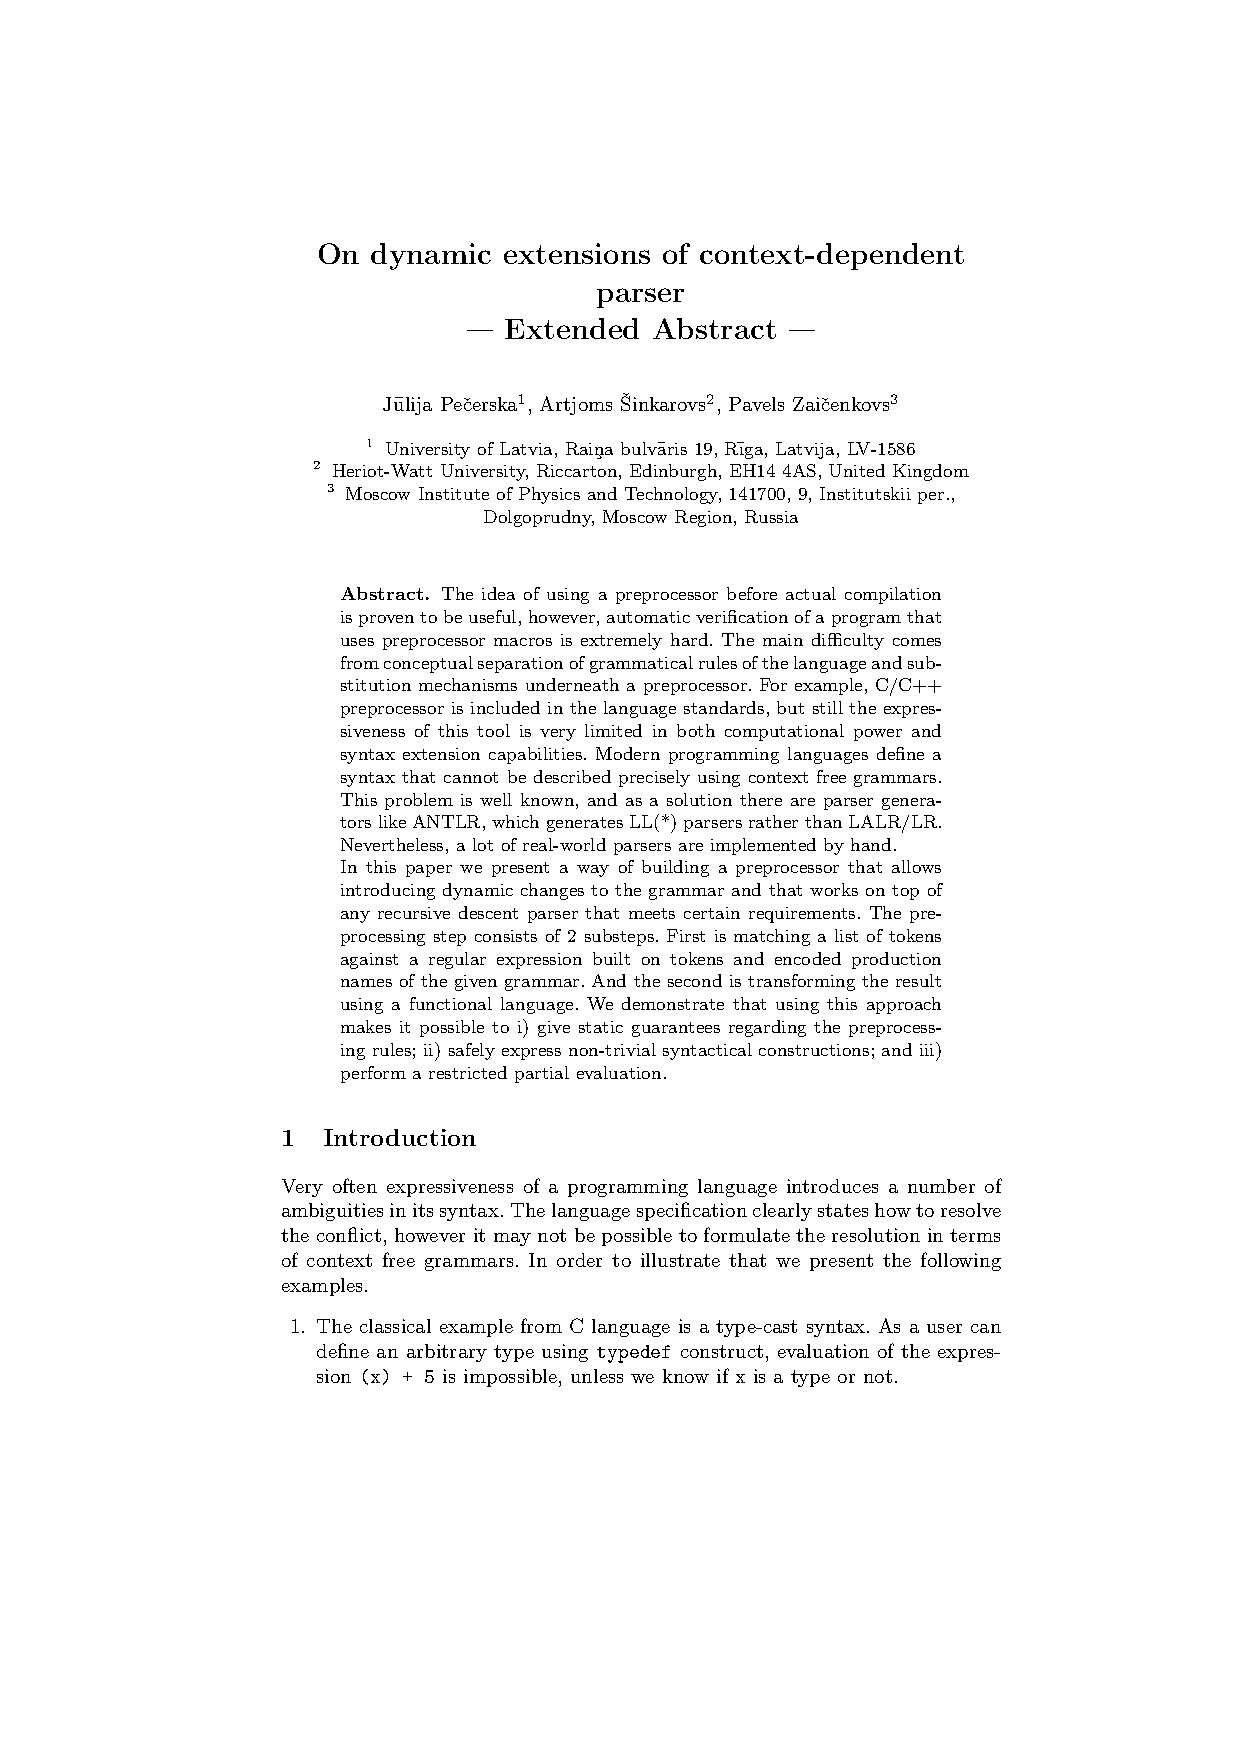
\includepdf[pages={-}]{paper/paper.pdf}

\end{appendices}

\bibliography{bachelors}{}
\bibliographystyle{plain}

\reglapa

\end{document}